\chapter{Introduction}
\label{chap:introduction}

% To fully understand our history, we would hope to understand 1. how we, individually, became conscious; 2. before that, how we developed into human beings; 3. before that, how life began on Earth; 4. before that, how Earth and the Solar system formed; 5. before that, how the Sun formed; and 6. before that, how the Universe formed. The first and final of these questions are generally beyond the scope of traditional Western science, although some neuroscientists and cosmologists (as well as religious scholars, seekers, and philosophers) still try. The second and penultimate questions - how the species (the host of our consciousness) and the Sun (the host of our bodies) came to be - mirror one another both poetically and in that scientists seem to have a fairly solid grasp on each of them, using Darwin's theories and the Hertzprung-Russell Diagram to chart the evolution of our species and our host star. At the center of these six questions, how Life and Earth came into being, we find another symmetry, perhaps most notably thanks to the fact that it is here that science and (Abrahamic) religion disagree most strongly: to the religious mind, the Earth and Life were divinely Created, drawn out from Nothingness into their current, stable forms, while to modern science, life seems to have been the result of some fortuitous chemical mixing and our home, the Earth, the simple by-product of an inefficient stellar formation process somewhere in the suburbia of a minor galaxy in an infinitely vast Universe, both still evolving and changing.
%
% This thesis is an exploration of a miniscule step in the modern Western science's process of finding an acceptable solution to the question of how the Earth and Solar System formed.


Planetary systems, including our own Solar System, are born from circumstellar disks of gas and dust around young stars. Young ($\leq$ 10Myr) circumstellar disks, known as protoplanetary disks, are easily distinguishable from their older siblings by their large abundance of gas, which typically outweighs the disk's dust by a factor of 100. However, as these disks age they are influenced by gravitational, chemical, and viscous forces, and their gas almost entirely dissipates as they become debris disks, much like our familiar local Solar System's Kuiper Belt and asteroid belt. But while we can observe with relative ease the current state of our local planetary system and debris disks, understanding the process that brought us here is much more difficult. To do so, we must understand the nature of our own disk at its birth, and whether or not that process is a common one that we would expect to see replicated elsewhere. Unraveling this mystery requires that we turn to observations of other comparable protoplanetary disks in order to develop a coherent narrative of disk evolution and, consequently, the conditions necessary for the formation of planetary systems like our own.

To understand the birth of our protoplanetary disk, we must understand the birth of our Sun, as the two are intimately related. Stars form when a region of a molecular cloud develops a gravitational instability sufficient to lead to a runaway collapse \citep{Shu1987}, helped along by macroscopic turbulence in the cloud \citep{MckeeOstriker2007}. In this process, the cloud shrinks by a factor of around ten million on its way down to a star, analagous to shrinking a square the approximate size of Connecticut ($\sim$150x150 km) down to just 15mm on each side. Angular momentum, defined as the product of a system's mass, velocity, and radial extent, must be conserved throughout this process,  leading to a tremendous increase in the collapsing cloud's angular velocity. As the local material begins to self-gravitate, its center forms a dense core which will eventually become a young star\footnote{binaries are also a common outcome in this process; according to \citet{DucheneKraus2013}, approximately half of all stars are found in binary systems.}.

However, if that angular momentum is conserved only through an increase in angular velocity, those velocities will become so large that the star itself will be unable to form, as centrifugal forces pulling outward will become more significant than the gravitation pulling the star in on itself. In order to prevent velocities from becoming this high, stellar jets and disks, made from the collapsing material, will develop to decentralize the system's mass and dissipate its angular momentum.

The resulting disks present flared radial structures, typically extending several hundred AU \citep{VicenteAlves2005}. Since these disks form directly out of the collapse process, they, like their stellar host and the initial molecular cloud, are initially composed almost exclusively of molecular hydrogen, although their chemical evolution is significant and heavily studied\footnote{Improving our understanding of this chemical evolution is also one of the motivating drives of this thesis.}. Temperatures in their outer reaches are typically in the range of 10-100 K; gas masses are inferred to range from ones to tens of Jovian masses \citep{AndrewsWilliams2005}, although this value comes with significant assumptions that are discussed in depth in \S\ref{section:continuum_emission}. Masses for the disks in the present study are calculated in Chapter \ref{chap:results}.


% Meredith:
% You should be more specific about what you mean here by “masses” — really what you mean is an inferred gas mass based on the observed dust flux, converted into a dust mass by an assumed opacity, and then into a gas mass by assuming a 100:1 gas:dust mass ratio.
%
% The three HUGE assumptions that go into this are:
% (1) we know the opacity, which really depends on three main unknowns:
%         - the dust composition
%         - the dust shape
%         - the dust size distribution,
% (2) we are seeing all of the solids, which is almost certainly untrue since an unknown amount is locked up into large, invisible bodies like planetesimals and planets,
% (3) we know the gas:dust mass ratio, which we probably don’t (there’s a whole literature on this, especially recently — Kamber Schwarz’s thesis papers, Ted Bergin’s HD observation of TW Hya, and Jonathan Williams’s student whose name I’m forgetting are a good place to start).
%
% Jonas:
% Establishing the masses of the disk's gas and dust is a multi-step process




\begin{figure}[htp]
  \hspace*{\fill}%
  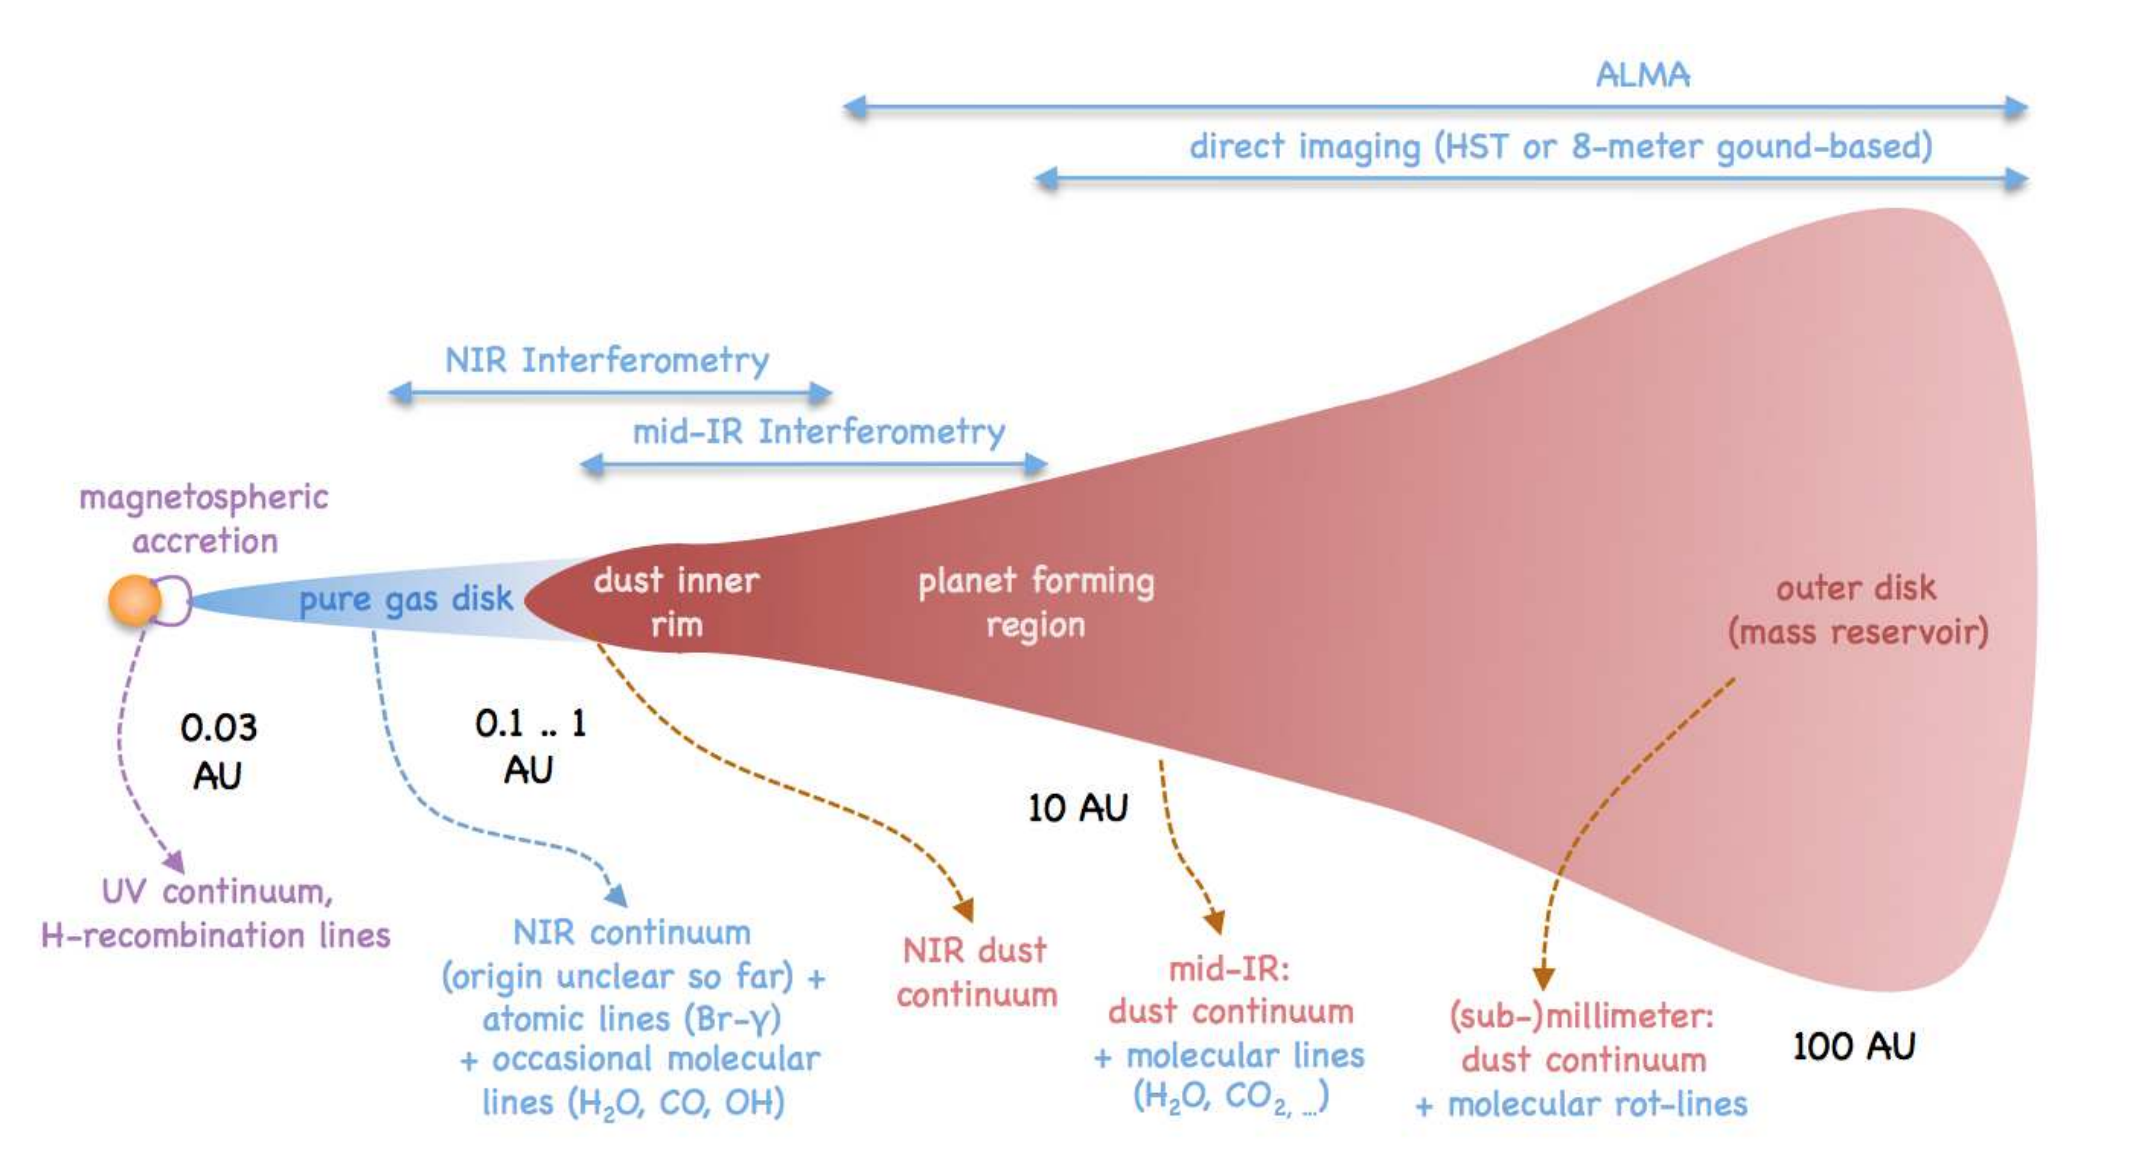
\includegraphics[width=\linewidth]{proplyd_structure.png}\hfill%
  \hspace*{\fill}%
  \label{fig:proplyd_str}
  \captionof{figure}{An edge-on slice of a protoplanetary disk is presented \citep{DullemondMonnier2010}. As is visible in this graphic, significant radial segmentation of the disk exists, particularly between the inner gas disk and outer disk of gas, dust, and planetesimals. Also of note is the large vertical flaring that occurs at large radii. Since the observations that this thesis are based on were made with ALMA (discussed in \S\ref{section:interferometry}), we are sensitive primarily to the outer reaches of the disk.}
\end{figure}



By around 10-20 Myr, the primordial gas and dust in these disks becomes depleted through several processes, including accretion onto the host star, blowing out from radiation pressure, and becoming locked up in icy bodies, transitioning the disk from a protoplanetary disk to a debris disk. These new debris disks are made up of what is thought to be second generation dust, created by the grinding down of boulders and planetesimals, since any primordial dust from the initial collapse should have been blown out by this time. The gas masses in debris disks tend to be orders of magnitude lower than in protoplanetary disks. For a more complete review of disk evolution, see \citet{Hughes2018}.




\section{Submillimeter Observations}

Although protoplanetary disks' masses are dominated by gas, they still have sufficient dust to be optically thick in the optical. Consequently, mass measurements are not possible at optical wavelengths. However, since the optical depth of the dust at millimeter wavelengths is low, and since the emission being observed at these wavelengths is thermal rather than due to scattering (as it is in the optical), observations at millimeter wavelengths are preferred for measuring a disk's dust mass. In the radio, we may trace two types of emission:

\begin{itemize}

  % How do you know that the dust doesn’t absorb at mm wavelengths??? If there’s mm-size dust, it should absorb mm wavelengths!  The small dust grains won’t, but remember that there’s a whole size distribution, and in fact, the balance between the steep size distribution (weighted towards small grains) and the dropoff of emission efficiency (weighted towards large grains) means that the grains we are seeing at mm wavelengths are most likely in fact the mm-size grains that *do* both absorb and emit efficiently at mm wavelengths.

  \item \textsc{Continuum emission}: Although the size distribution of grains in a dust disk is wide and heavily weighted towards smaller grains, larger, millimeter-sized grains are still present in disks. These larger grains are far more efficient emitters in the radio, since the wavelength of a grain's peak thermal emission efficiency is approximately equal to its size. Thus, we may observe this continuum emission (so named thanks to the wide range of frequencies that thermal emission covers) from these millimeter-sized grains.

  % I think it might be good to be specific here that continuum emission is (1) from dust, and (2) thermal in nature (which is why it spans a wide range of frequencies)

  % I don't like this, but maybe it's fine
  \item \textsc{Line emission}: Because radial disk temperatures quickly fall below the temperatures required to cause photodissociation, molecules may live a stable existence in these disks. Conveniently, the rotational transitions of small molecules tend to emit at radio frequencies. Observations of the emission from these rotational transitions, known as line emission, can provide us with a wealth of important information, including kinematics, temperature information, disk chemistry and total disk mass.
\end{itemize}


Notably absent in both forms is emission from the central star, thanks to the fact that stars are extremely weak emitters in the radio regime, since stars are hot and, consequently, have peak emission in the optical\footnote{Why, then, is the dust still bright relative to the star? While it's true that the flux \textit{per area} of the dust is significantly smaller than of the star, the dust has a far greater surface area, allowing it to compensate and still be a bright emitter.}. This makes them very faint relative to the disk's emission at longer (hundreds to thousands of microns) wavelengths. Fig \ref{fig:SED} \citep{Hughes2010} presents a spectral energy distribution, or SED, showing emission intensity as a function of wavelength from an imaginary disk system, demonstrating how small the star's flux density is at long wavelengths relative to the disk's contributions.


\begin{figure}
\centering
  \includegraphics[width=\linewidth]{Meredith_SED.png}
  % 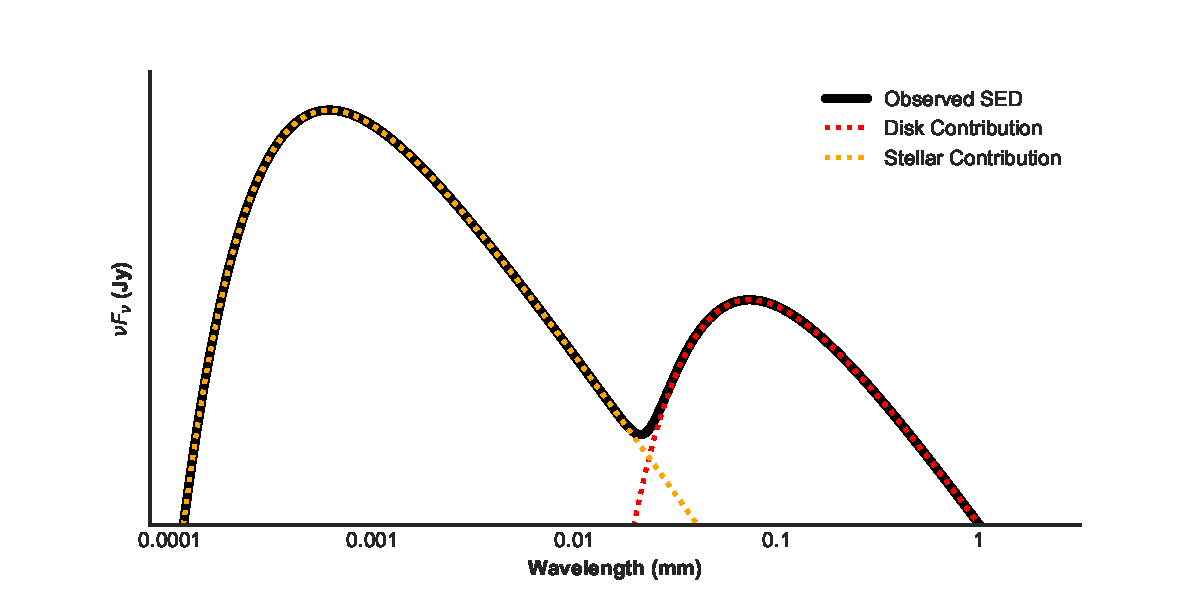
\includegraphics[width=\linewidth]{example_SED.pdf}
  \captionof{figure}{Two example SEDs, accompanied by cartoon models to illustrate the various contributions of different elements of a disk and their influences on the SED \citep{Hughes2010}. The dashed line corresponds to emission from the stellar photosphere, while the colored lines are blackbody curves corresponding to emission from regions of the disk with different temperatures. Since radio observations take place at longer (hundreds to thousands of microns) wavelengths, one may easily see that the stellar contribution in that regime is minimal.}
  \label{fig:SED}
\end{figure}

% Meredith's caption: Cartoon illustrating SED modeling and the association between midIR deficits and inner holes in transition disks. The black solid line shows a model of a T Tauri star surrounded by a disk that (left) extends in to the dust destruction radius or (right) is truncated at 1 AU from the star. The dashed line marks the SED contribution from the stellar photosphere. The colored lines are blackbody curves showing the contribution of dust at different temperatures to the excess over the photosphere: curves with peaks at shorter wavelengths originate from hotter dust. The mid-IR deficit in the figure on the right corresponds to missing emission from the hottest dust. The illustration below each plot shows how the temperature of the dust is related to distance from the star, and highlights the idea that missing short-wavelength emission from the SED corresponds to missing dust close to the star

However, to understand these types of observation, one must first understand the nature of the ``telescope" making the observations. What follows is a brief introduction to radio interferometry, followed by more complete explanations of continuum and line emission.



\subsection{Interferometry}
\label{section:interferometry}
Interferometry is a clever way to make extremely high-resolution observations at long wavelengths without needing to use incredibly large collecting areas. Were one to naively attempt to create a ``traditional" (single-aperture) telescope to capture radio emission, they would quickly recall that, for a telescope with a single circular aperture of diameter $D$, maximum angular resolution is given by
% Ignoring a Meredith comment here about this being a general equation if we replace D with a baseline.
\begin{align}
  \theta &= 1.22 \, \frac{\lambda}{D},
\end{align}

\noindent where $\theta$ is the angular resolution achieved, and $\lambda$ is the wavelength of the emission being observed. Unfortunately, light in the radio regime has wavelengths on the order of millimeters to centimeters, orders of magnitude longer than optical light, which is in the hundreds of nanometers. Consequently, to achieve a resolution comparable to that of an optical telescope, one would have to increase their aperture's diameter accordingly to match the increase in $\lambda$. Some have tried this approach: the Arecibo Observatory in Puerto Rico and the Five hundred meter Aperture Spherical Telescope in China (with diameters of 300m and 500m, respectively) are two immediate examples, but both still have resolutions ($\sim25''$ for Arecibo and $\sim15''$ for FAST, observing 3cm emission) that are too coarse to resolve the length-scales that we would like when observing disks. Building and maintaining apertures this big is also an extreme challenge, usually requiring mountains to be hollowed out, making this an unappealing solution.

%REWORK: Make sure to note that ALMA has lots of big dishes so sensitivity is less of an issue.

The alternative is to leverage the power of interferometry for a solution to the problem. In an interferometric system, one may construct an image using the interference patterns between light received by two or more separate apertures. In this case, the maximum angular resolution becomes inversely proportional to the maximum distance, or \textit{baseline}, between any two  apertures, which can be made almost arbitrarily large. Interferometry does come with tradeoffs, however, the most notable of which is in sensitivity, since sensitivity is proportional to collecting area and each dish in an interferometer is typically fairly small. Additionally, inteferometers also have inherent spatial filtering, meaning that they are not sensitive to flux from sources covering large angular scales. This is because the largest angular scale of a flux source that a telescope is sensitive to is inversely proportional to its smallest baseline. Since the collecting area of a single-dish telescope is a continous surface, its smallest ``baseline" is essentially infinitely small (making it sensitive to arbitrarily-large flux sources). Conversely, for an interferometer, that smallest baseline is typically ones to tens of meters. Therefore, interferometers are intrinsically unable to capture flux from sources with angular scales larger than $\lambda/D_\text{min}$.\footnote{This can actually be an advantage, however, as it offers the opportunity to choose the length-scale being observed, i.e. remove cloud contamination (large scale structure) from an image of a disk (a small structure).}


% Well, it’s only unappealing if you don’t also need the collecting area.  There are certainly advantages to single apertures, chief among them sensitivity, as well as the ability to measure total fluxes (which is why we often want to try to get single-dish flux measurements of ALMA sources, though that doesn’t work in the case of Orion because there’s too much cloud contamination).  IGNORING THIS

% In our case, the resolution is important because disks have angular scales that are too small to resolve with single-dish telescopes, and interferometry also happens to be convenient for highly contaminated molecular cloud regions like Orion — spatial filtering is often listed as one of the drawbacks of interferometers (because we miss flux on large angular scales), but in our case it’s a benefit because it lets us be sensitive to the relatively small-scale structure of the disk while ignoring the large-scale structure of the cloud that would overwhelm a single-dish telescope.

% The tradeoff is lower sensitivity, but ALMA mitigates that somewhat with its large number of dishes (the LNSD design is becoming the gold standard for interferometers, though ALMA’s dishes can’t really be said to be small… though again, that’s not an issue for us, since we don’t need a large field of view to look at tiny disks.  It’s certainly a drawback of interferometry for galaxy observers, though!)



While this interference process can be done at optical wavelengths with CCDs, it is far more difficult to execute, as light must be forced to physically interact before reaching the sensor via a complex and extremely precise optical system. At longer wavelengths, however, heterodyne receivers may be used, making the task of interfering the signals a digital process, rather than a physical one. A heterodyne receiever records both the amplitude (analogous to the intensity that a CCD might measure) and the phase of the signal it receives. Because the receiver captures phase information as well as amplitude, the signals from two dishes may be digitally interfered after being received. Physical features must be calibrated out, including phase delay caused by differences in line-of-sight path length from the source between the receivers, atmospheric effects, and instrumental phase delays. The result, for a single baseline, is a complex voltage pattern describing the amplitude and phase of the interference pattern between the signal each dish received. We call this voltage pattern a \textit{visibility}.


% “is called a visibility and lives in the visibility domain” — just think of how incomprehensible this sentence would have been to you three years ago. :-)

% Maybe start this paragraph with a general statement that what an interferometer records is actually the Fourier transform of an image, and that the visibility domain is the Fourier transform of the image domain.  

The complete output from an interferometer is a collection of these visibilities. Taken together, they approximate the Fourier transform of the sky image. We say that this output lives in the ``visibility domain", which itself is a Fourier transform of the image domain. A single visibility relates to the full set of visibilities analogously to the relationship between a pixel and an image.


While the image domain has spatial dimensions (i.e. the $xy$ plane), the visibility domain instead uses the $uv$ plane. The $uv$ plane is a wavelength-scaled $x-y$ coordinate system parallel to the sky in the direction of the target source. Here ``wavelength-scaled" can be taken to mean that $u = X/\lambda, v = Y/\lambda$, where $\lambda$ is the wavelength of observation and $X$ and $Y$ are the lengths of the $x$ and $y$ (i.e. north/south, east/west) components of the projected baseline. Thus, each baseline samples a specific spatial frequency, given by $\theta = 1/\sqrt{u^2 + v^2}$. An interferometer may thus be represented on the $uv$ plane as a scatter of points, with each point corresponding to the wavelength-scaled, target-projected, component distance between two receivers. The ideal aperture would completely fill the $uv$ plane, so that every spatial frequency was sampled. However, since the number of baselines we may access is very limited (approximately the square of the number of antennae in an array), this is clearly an impossibility for an interferometer.\footnote{Of course, a single-aperture telescope does not have this problem since its $uv$ plane is one continuous collecting area and thus can be seen as having infinite baselines and complete $uv$ coverage.}


However, the fact that the $projected$ baseline is really what determines visibility's location in the $uv$ plane, rather than the baseline's ``true", un-projected length, allows us to cleverly gain far more points in the $uv$ plane than one might immediately expect. Since the Earth rotates throughout the night, the projection of a given baseline relative to the target source will change throughout the night as well. Consequently, by making observations over the course of a night, many more points in the $uv$ plane may be sampled, yielding a better-filled plane. This process is known as ``Earth rotation aperture synthesis."

We now consider how one might recover an image from a set of observed visibilities. In general, moving between frequency space and distance space is given by a simple Fourier transform. When applying this translation to telescopes, we consider the shape of the image produced by observation of a single point source directly on axis with the aperture. For a conventional telescope with a circular aperture, coverage in the $uv$ plane is in the shape of a filled circle of constant amplitude. Translation to the image domain, via a Fourier transform of that shape, results in the familiar 2-D Airy Disk, the characteristic point-spread function (PSF) of a single aperture convolved with a point source. With an interferometer, this process would be equally straightforward if the $uv$ plane were fully sampled, but because it is not, the resulting image is instead a Fourier transform of all the points in the $uv$ plane sampled by the baselines, and can take on a very complex shape\footnote{Additionally, thanks to the incomplete sampling of the $uv$ plane, an infinite number of images could all be consistent with some given finite set of visibilities, although many of them would not be physically possible. The one we choose to look at is determined by our deconvolution process, but is not actually the true image.}. However, while this shape is complex, it is still - as is the case in the optical - just a convolution of the point source with some PSF, only in this case the PSF is more complicated than an Airy function. As we increase the number of $uv$ points sampled, the resulting image will increasingly approximate a bumpy and/or elongated Airy disk. In radio astronomy, we call this PSF the ``dirty beam".

% For above: “can take on a very complex shape” — I wonder if it would be helpful here to introduce the concept of the PSF (or dirty beam) and the fact that the raw image is in fact the convolution of the true image with the PSF (this is true for all telescopes, not just interferometers, so it can be a helpful concept for optical astronomers trying to figure out interferometry).  

When observing a source, we would like to find the true sky brightness pattern (i.e. the sky image). As described above, the Fourier transform of a set of visibilities is a convolution of the dirty beam with the true sky brightness pattern. Therefore, we would like to remove the dirty beam's contributions to the image. The process of removing the influence of the dirty beam, and the artifacts it can introduce, is called deconvolution. In practice, this deconvolution process takes the form of some iterative algorithm that selectively removes the effects of the dirty beam. The curious reader is referred to the CLEAN algorithm \citep{Hogbom1974}, the first and most popular deconvolution algorithm (and the one used in this work), as well as the maximum-entropy method \citep{Wernecke1977,SkillingBryan1984}. It is worth noting at this point, however, that due to the artifacting and non-unique result that the imaging process introduces, all of our analysis is performed directly on the visibilities themselves, rather than the image. This means that the specific parametrization of CLEAN or any other step in the imaging process does not need to be perfect, since it is purely diagnostic or expository.


In summary, interferometry works by recording amplitude and phase information about some emission with many radio antennae and digitally interfering each antenna's signal with the signal received by every other telescope. Each of the resulting interference patterns is called a visibility, and represents a point in $uv$ space. Translation from the visibility domain to the image domain involves taking the Fourier transform of the visibilities and deconvolving the dirty beam's influence.

Currently, the world's most advanced interferometer, and the source of this thesis's data, is the Atacama Large Millimeter/Submillimeter Array (ALMA), shown in Fig \ref{fig:ALMA}. Built in the high Chilean desert at around 5,000 meters (16,000 feet), the \$1.4-billion array first opened its eyes for scientific observation in mid-2011, with funding from a global partnership between Chile, the United States, and several other countries. With its 66 total antennae (50 12-m dishes and 16 7-m dishes) and baselines extending out to 15-km, it offers an order of magnitude increase in sensitivity and resolution over previous arrays that observe at similar frequencies, which include the Submillimeter Array (8 6-meter dishes), NOEMA (10 15-meter dishes) and the CARMA (23 dishes of 3.5-m, 6.1-m, and 10.4-m diameters).

\begin{figure}[htp]
  \hspace*{\fill}%
  \subcaptionbox{\label{fig:ALMA}}{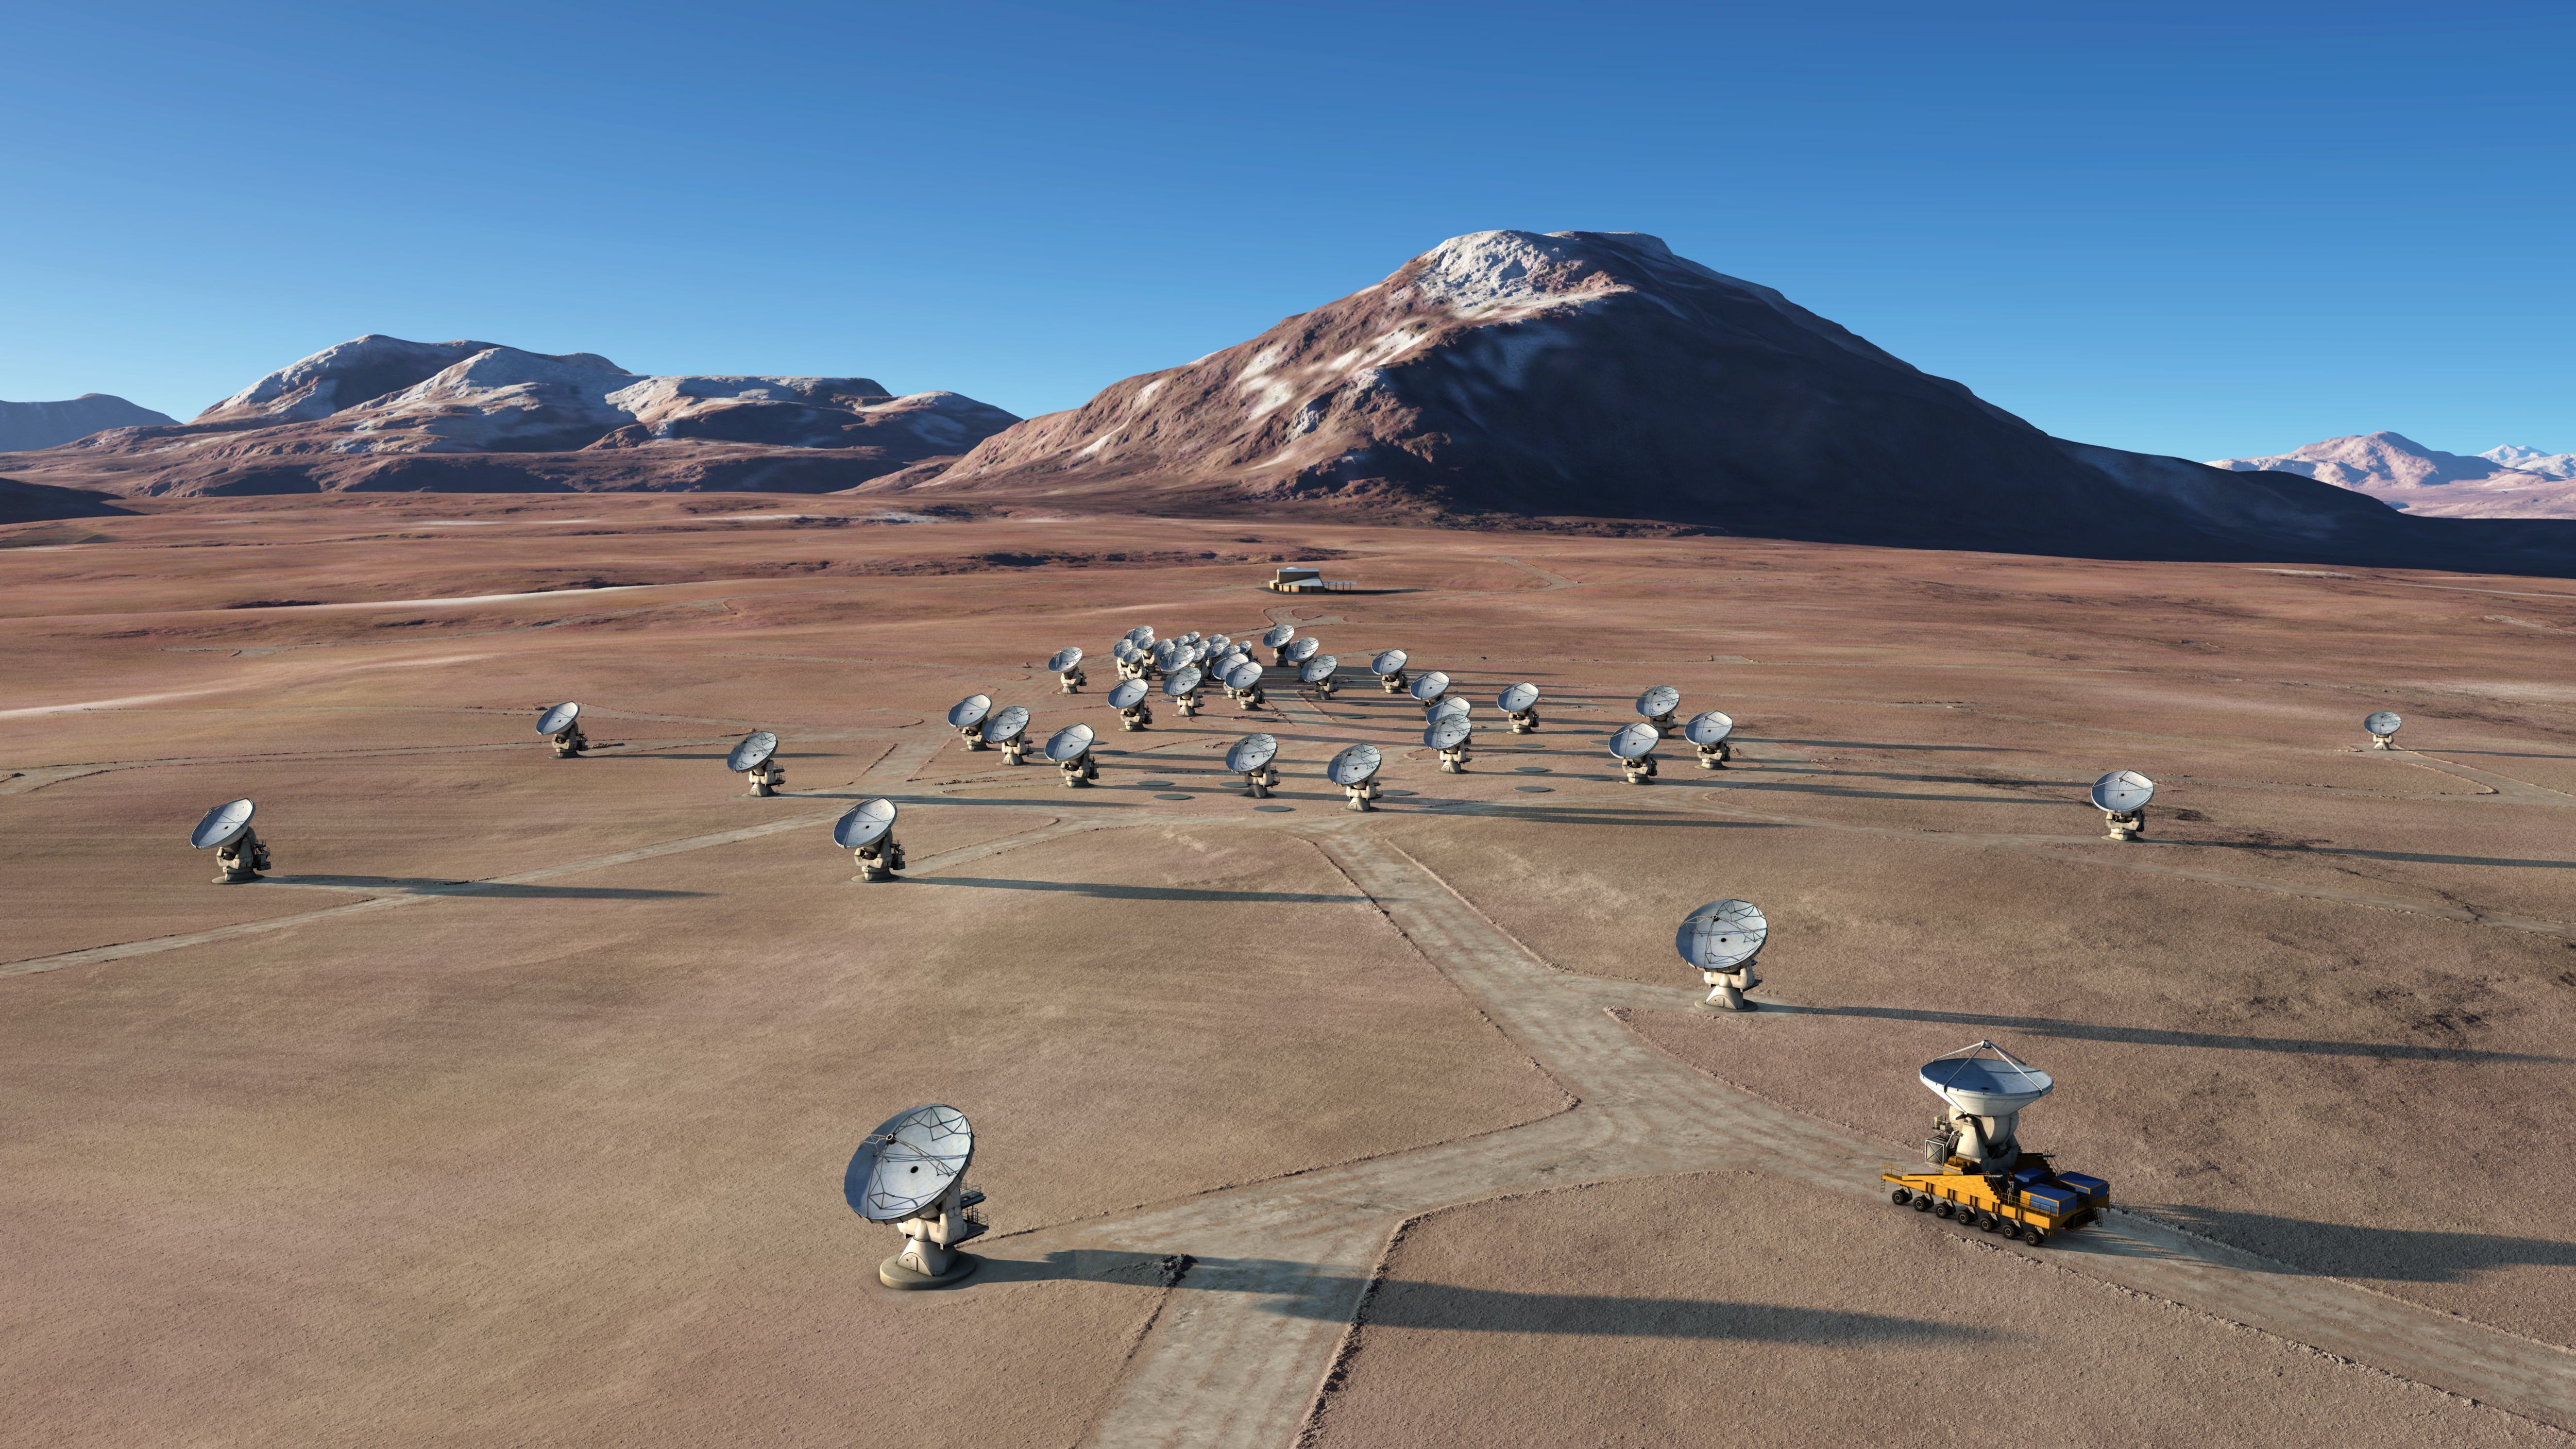
\includegraphics[width=0.5\linewidth]{ALMA_universetoday.jpg}}\hfill%
  \subcaptionbox{\label{fig:Andrews_proplyds}}{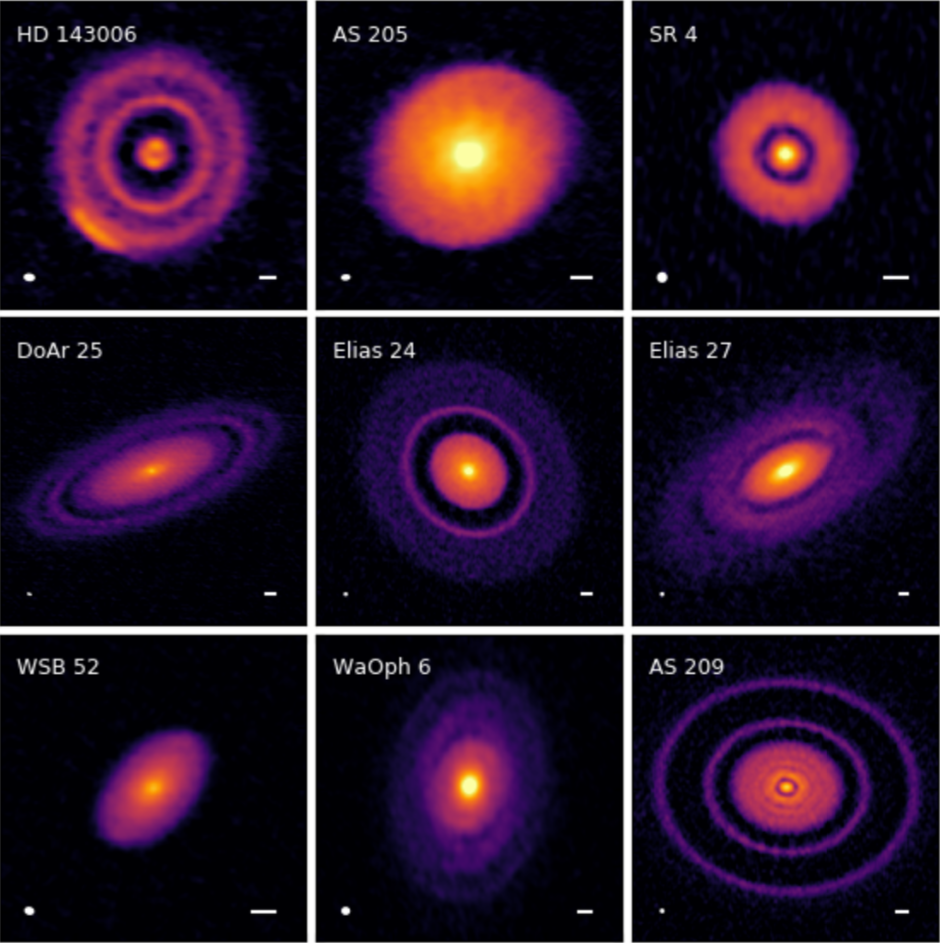
\includegraphics[width=0.3\linewidth]{Andrews2018_proplyds.png}}%
  \hspace*{\fill}%
  \captionof{figure}{\textit{Left:} A rendering of ALMA\footnote{Courtesy of \url{www.almaobservatory.org/en/about-alma-at-first-glance/origins/}} shows the interferometer's antennae in the high desert, as well as a purpose-built truck moving one of the antennae (lower right). \textit{Right:} A recent survey from ALMA by \citet{Andrews2018} reveals stunning detail in several protoplanetary disks.}
\end{figure}


The effects of this increase are impressive; gaps and rings in faraway disks are now resolvable in striking clarity (Fig. \ref{fig:Andrews_proplyds}), providing a treasure-trove of opportunity to hone our understanding of disk evolution and planetary-system formation. ALMA has also been a blessing to other subfields of astronomy as well, enabling high-resolution observations of everything from complex organic molecules in disks \citep{Walsh2016,Podio2019} to gravitational lensing from dark matter halos \citep{Herrera-Martin2019} to molecular tori around black holes \citep{Combes2018}. Additionally, as a component of the Event Horizon Telescope, ALMA played a key role in imaging a black hole's event horizon for the first time \citep{EHTCollab2019}. These awe-inspiring projects are a small portion of ALMAs contributions to the world of radio astronomy, and more are being made with each passing day.


With an improved understanding of the mechanics of radio interferometry, we may now revisit continuum and line emission.

% \begin{figure}
% \centering
% \begin{minipage}{.48\textwidth}
%   \centering
%   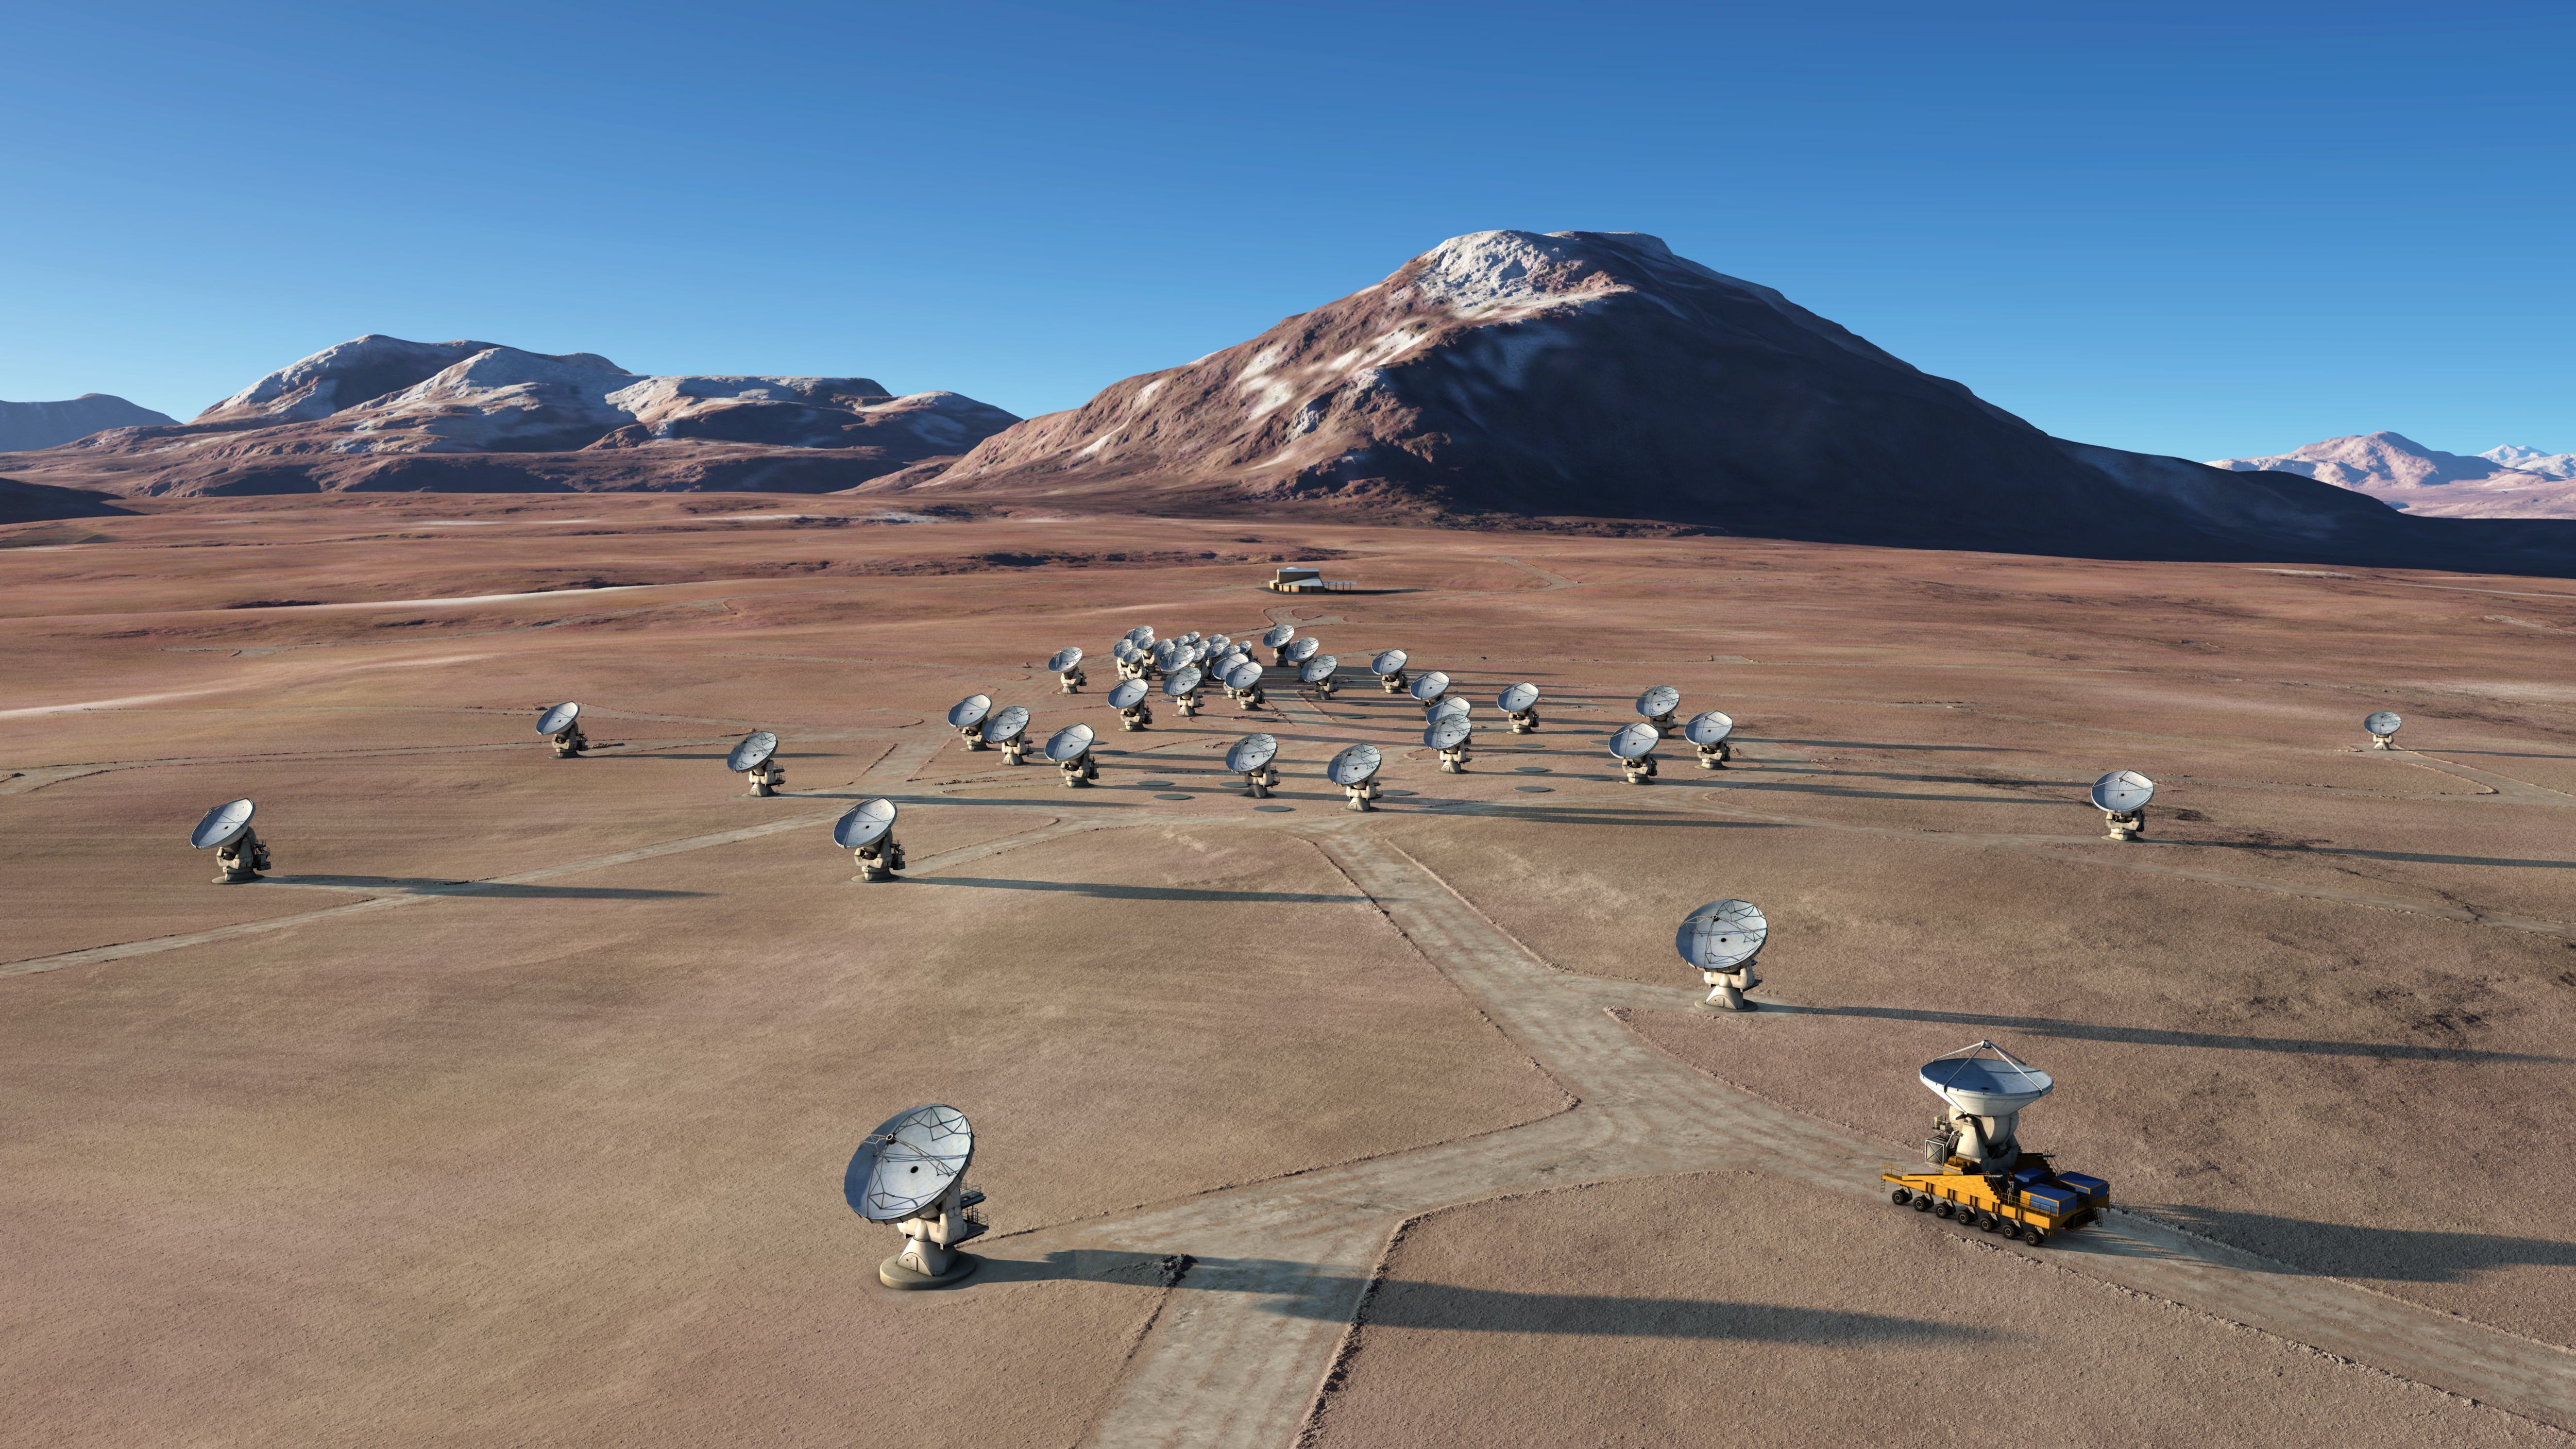
\includegraphics[width=\linewidth]{ALMA_universetoday.jpg}
%   \captionof{figure}{A rendering of ALMA. Antennae may be moved using a large truck, as seen in the lower right corner.}
%   \label{fig:test1}
% \end{minipage}%
% \begin{minipage}{.27\textwidth}
%   \centering
%   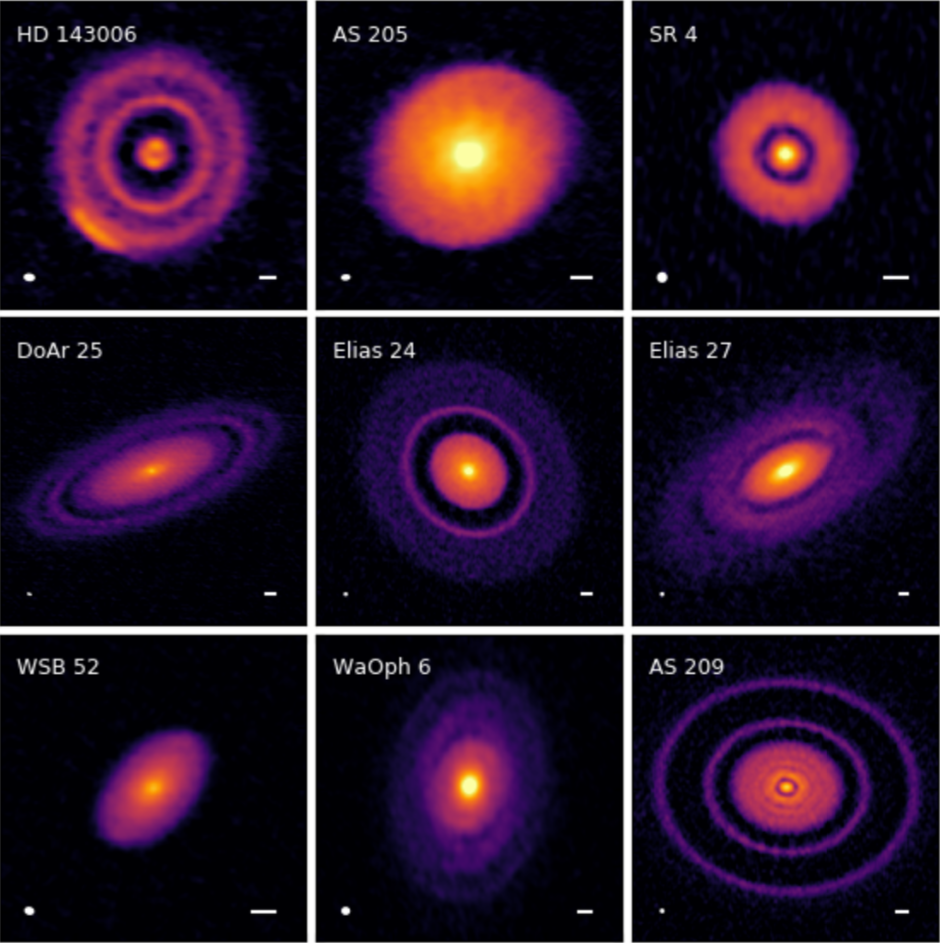
\includegraphics[width=\linewidth]{Andrews2018_proplyds.png}
%   \captionof{figure}{Impressive images of disks from Andres et al (2018)}
%   \label{fig:test2}
% \end{minipage}
% \end{figure}




\subsection{Continuum Emission}
\label{section:continuum_emission}

Continuum emission observations integrate flux from a wide band of frequencies, just as our eyes do in the optical. They are appealing for their simplicity and because, by integrating a wide band, they are sensitive to faint objects.

When observing protoplanetary disks, an understanding of planet formation is often a guiding motivation. One parameter that is critical to the planet-forming process is total disk mass. We know that, to first order, when a disk is optically thin, its total mass, $M_{\text{disk}}$, is linearly proportional to its flux density, $F_{\nu}$ \citep{Hildebrand1983}, which is found from an observation of continuum emission. This relationship is given by

\begin{align}
M_{\text{dust}} = \frac{F_{\nu} d^2}{\kappa_{\nu}\ B_{\nu}(T_c)},
\end{align}

%below: really opacity power law index, but simpler this way and they mean the same thing.
where $d$ is the source's distance, $\kappa_{\nu}$ is an assumed dust opacity, and $B_{\nu}(T_c)$ is the Planck function at a given charatcteristic temperature, $T_c$. The value of $T_c$ and disk opacity can be inferred without much difficulty by fitting the disk's SED using a simple model. This function is, of course, rather approximate; it assumes a single temperature and single dust opacity (a function of composition and grain size distributions) throughout the disk. The assumption of optically thin emission means that calculations made will inherently be lower limits, since any substantial optical depth will block emission from inner regions of the disk. Futhermore, even in the case of optically thin emission, significant mass may be locked up in bodies that are invisible to our observations.

Traditionally, studies have used observed continuum fluxes to estimate dust mass and then inferred a total gas mass by assuming a 100:1 gas/dust ratio, based on the ratio observed in warm ISM clouds. However, an ALMA survey of 89 disks in Lupus tracing both continuum emission and two CO isotopologues \citep{Miotello2016,Miotello2017} found the true value of this value to be highly variable, often falling closer to 10 (Fig \ref{fig:gas-dust-ratios}), and \citet{Liu2018} found that a ratio of 100 provoked instability (as measured by the Toomre criterion) in their smoothed-particle hydrodynamic simulation of the MWC 480 disk; instead, they found that values of 6-12 yielded their best results. \textit{Could cite Bergin+ 2013 here for coming up with the HD stuff, but not sure how to make it work narratively.} In short, this ratio introduces a significant source of uncertainty, possibly of up to two orders of magnitude, into existing calculations of gas mass in protoplanetary disks based that are based on continuum emission.



\begin{figure}
\centering
  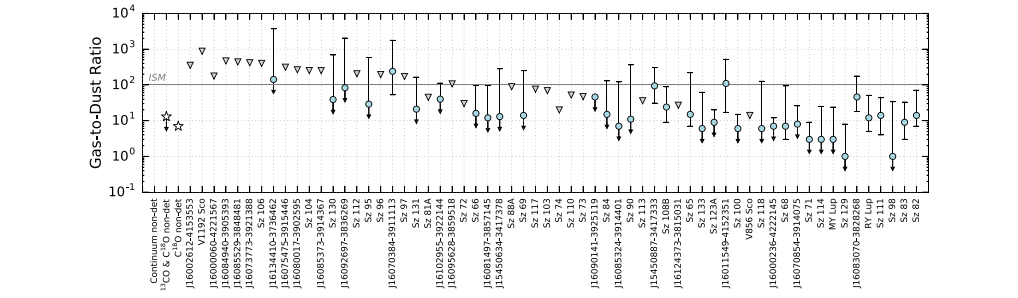
\includegraphics[width=\linewidth]{gas-dust-ratios_Miotello16.png}
  % 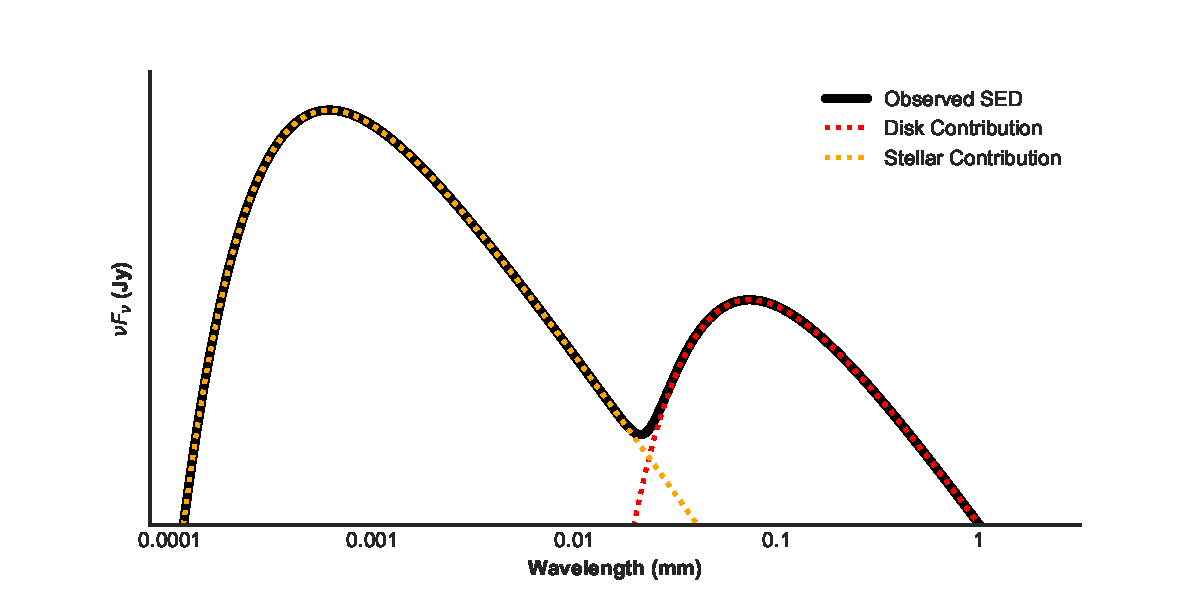
\includegraphics[width=\linewidth]{example_SED.pdf}
  \captionof{figure}{Gas-to-dust ratios in protoplanetary disks in Lupus \citep{Miotello2016}. The ratio is highly variable and rarely best described by the canonical value of 100:1. Blue points indicate detections, and gray triangles indicate upper limits. Error bars with downward arrows indicate sources detected in $^{13}$CO but not C$^{18}$O, for which the authors did not establish lower mass limits.}
  \label{fig:gas-dust-ratios}
\end{figure}







\subsection{Line Emission}

As molecules collide with one another or absorb light, they gain energy, entering higher rotational energy states. However, as their presence in these states cannot be sustained without the addition of more energy, they will de-excite soon after. This de-excitation process - stepping down from one rotational energy state to the one below - causes the emission of light. Every transition in every molecule emits at its own specific frequency, or rest frequency, making that light identifiable to observers. We may observe a specific rotational transition from a single type of molecule by tuning our receiver to be sensitive to a very narrow window of frequencies immediately around the rest frequency of the transition of interest. This is known as a spectral window. The narrow range of frequencies at which a given molecular transtion emits makes ALMA's large sensitivity particularly crucial for observations of molecular lines at high spectral resolution or in rare species.

One immediate feature that line emission gives us access to is velocity information: since all emission should have a single frequency (the transition's rest frequency), we immediately know that any variation from that central frequency is a result of Doppler shifting caused by line-of-sight velocity\footnote{Technically, the uncertainty principle tells us that a line will have some ``natural" width, but this width is small compared to the Doppler width.}. This allows us to make a ``moment-one" map of emisison, which shows the intensity-weighted velocity structure of the disks (Fig \ref{fig:ex_mom1}).


\begin{figure} %[t!]
\centering
  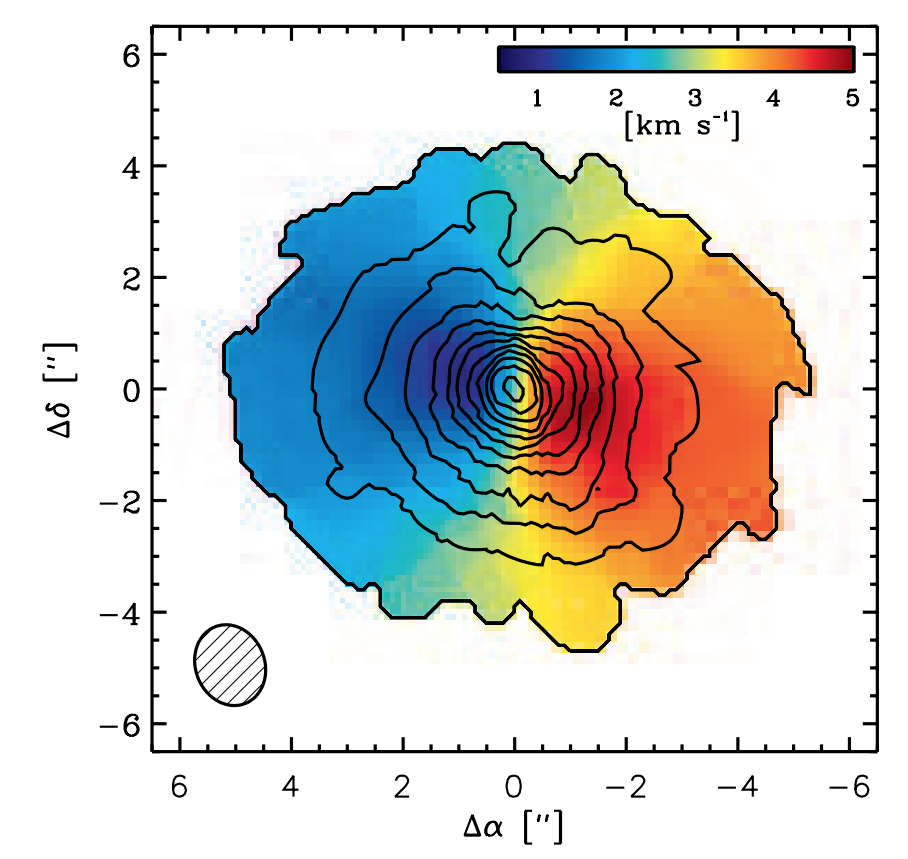
\includegraphics[width=\linewidth]{example_m1_image.png}
  \caption{An example of a moment-one map of a protoplanetary disk, drawn from \citet{Rosenfeld2012}. Colors correspond to intensity-weighted velocity; in other words, how quickly material is moving relative to the observer. One may consider this analogously to a spinning Frisbee, approaching the reader edge-on, where one half of the disk is spinning outwards (away from us) as the other side approaches. From this image, we immediately gain several pieces of information: for example, in this case, the disk as a whole is receding from view (since the velocity's "zero point", in yellow/green, is moving at 3 km/s), and that the disk's eastern half is spinning away from us, while the western half comes towards us. This gives us a quick understanding of the disk's kinematics.}
  \label{fig:ex_mom1}
\end{figure}


% Ignoring this from Meredith: (or multiple isotopologues, ideally, but we don’t have that in this case)
Observations of line emission also give us information about both the temperature and density structures of the disk, since these are the two factors that influence how much emission we observe. However, in the case of optically thin emission, the two are degenerate, since an increase in either one will increase emission intensity. In this case, we may combine observations of multiple species to model the temperature structure of a disk. In the case of an optically thick line, however, the temperature and density are no longer degenerate, since all emission originates from the $\tau=1$ surface, which removes density from the equation and gives us a value for the temperature at that point in the disk's vertical structure. This is valuable, since the a disk's vertical temperature profile varies significantly, with the surface notably warmer than the midplane.

Besides offering information about radial density and temperature profiles, line emission also provides another way of finding total disk mass. Like the initial cloud that the star and disk formed from, the vast majority of the disk's mass comes in its gas, and like that initial cloud, the vast majority of that gas is molecular hydrogen, or H$_2$. However, since H$_2$ is a symmetric molecule and thus has no permanent dipole moment, it has no rotational transitions and does not emit in the radio, making it invisible to our instruments. As a consequence, we must instead observe emission from other molecules, make assumptions about those molecules' abundances relative to H$_2$, and extrapolate the total disk mass.


To do so, one generally begins with CO, second most abundant molecule behind H$_2$. Thanks to its abundance, as well as its relatively low excitation temperature, CO provides robust, bright emission. Drawing on measurements of CO/H$_2$ ratios in warm dense cloud \citep{AikawaHerbst2003,Fogel2011}, we use a ratio of 1:10000, or 10$^{-4}$, to represent CO's relative abundance in protoplanetary disks, while for other, more complex molecules, relative abundances are generally drawn the interstellar-medium literature and chemical modeling.

However, this CO/H$_2$ ratio of 10$^{-4}$, which is frequently used to calculate total disk gas masses \cmmnt{(e.g. \citet{Ansdell2017})} comes with significant uncertainty. Using a gas-grain chemical model \citet{Reboussin2015} showed, through an analsysis of CO isotopologues, that at low temperatures (below 30-35K), CO is converted to less volatile molecules (typically s-CO$_2$ or s-CH$_4$). This means that below these temperatures, relative CO abundance quickly falls about two magnitudes below the literature value of 10$^{-4}$. \citet{Schwarz2016} followed this modeling with high spectrospatial resolution ALMA observations of four CO isotopologues in the nearby protoplanetary disk TW Hya, and confirming a ratio of C/H$_2 = 10^{-6}$. Additionally, \cite{Yu2017} notes that CO depletion in the outer disk and optically thick emission from the inner disk has lead observers (e.g. \citet{Ansdell2017}, who found surprisingly low disk masses in their survey of ONC proplyds) to underestimate disk mass by more than an order of magnitude if they assume CO/H$_2 = 10^{-4}$ and optically thin emission. They and \cite{Cleeves2015} also note that CO abundances change on short ($\sim$ 1 Myr) timescales, resulting in a degeneracy between disk age and mass. Ultimately, CO's tight dependence on disk temperature and its evolutionary trends with age increase the need for a well modeled temperature profiles to inform the selection of an appropriate molecular abundance of CO.



\section{Disks \& The Role of Environment}


%REWORK: This is a rough transition from that CO talk.

There is significant evidence that most stars in our galaxy \citep{LadaLada2003,Mann2015}, including our own Sun \citep{Gaidos2009,Tachibana2006}, formed in high-mass star forming regions, or HMSFRs. Therefore, understanding our own creation story necessitates the understanding of protoplanetary disk evolution in these SFRs, and the role that environment plays in that process. However, until ALMA came online in 2012, line-emission studies of disks in these HMSFRs were not feasible, due to the need for increased sensitivity and resolution in the observations.

Now that this telescope is available, however, HMSFRs are open for observation. We may use this opportunity to try to better understand the role that environment plays in the development and evolution of protoplanetary disks, comparing them to the well-studied disk population in low-mass \citep{AndrewsWilliams2005,Mann2015} and the one well-characterized disk in an HMSFR \citep{Factor2017}, and evaluate how that environment may affect planet-formation potential.

% Charles/Elizabeth Lada for star formation in HMSFRs
% Star formation reviews; check Protostars and Planets VI


\subsection{The Minimum Mass (Extra-)Solar Nebula}

The minimum-mass solar nebula (MMSN) is a conceptual aid used to inform astronomers about the distribution of material required to form a planetary system \citep{Weidenschilling1977}. The MMSN is the radial mass profile that our own Solar System would present if the mass of each planet were, rather than being bound up in spheres, instead ground up and spread across the ring bound by the orbits of their inferior and superior neighbors. Gas is then added to the ring until the its gas:dust ratio reaches the canonical interstellar-medium value of 100:1\footnote{This ratio is discussed more in \S\ref{subsection:continuum}} (meaning that gas giants like Jupiter would have very little gas mass added, while terrestrial planets like Earth would have their mass significantly increased). The resulting mass profile represents the minimum surface density required to form our own protoplanetary disk and thus a way to inform our comparisons of other disks to our own. When this surface density profile is integrated into a single mass, it gives $M_\text{MMSN} = 0.01 M_{\odot}$.

It is, of course, an extremely approximate characterization. One significant assumption it makes is that our planets formed in their current positions. This is a statement that we know both to be false \citep{Walsh2011,Tsiganis2005} and consequential, since planetary migration can cause disks to lose mass by pushing competing planetesimals either out of orbit or into inner regions of the disk where they may be more susceptible to accreting onto the host star. Another assumption being made is that the chemistry is radially and temporally constant, which is also known to not be the case \citep{vanDishoeckBlake1998}.

The MMSN model was generalized to be tolerant to a wider diversity of planetary systems by \citet{Kuchner2004} as the minimum-mass extrasolar nebula (MMEN), using 26 Doppler-detected planets in multi-planet systems to construct a disk analogous to that of the MMSN. \citet{ChiangLaughlin2013} developed a similar model, this time drawing on Kepler and HARPS planets ($n \approx 10^5$) to explain the existence of close-in ($P < 100$ days) super Earths, which make up approximately half of the planets observed in those catalogues. Both models assume that planets formed at or near their current positions. However, \citet{Raymond2014} showed, using 191 multi-planet systems primarily drawn from the Kepler catalogue, that the resulting range of surface density profiles was broad, and thus that using a single, ``universal" profile to locate disks with planet-forming potential - as the MMSN/MMEN purports to offer - was not plausible. They note that this broad spread likely reflected the necessity for consideration of planet migration, particularly amongst gas giants.

Still, while the MMSN clearly makes significant assumptions that lead to inconsistencies, it is nonetheless used as an approximate barometer for planet-forming potential.




\subsection{Low- and High-Mass Star Forming Regions}
Thanks to limitations in sensitivity and resolution, most submillimeter surveys in the pre-ALMA epoch focused on young disks in the nearby low-mass SFRs of Taurus-Auriga and $\rho$ Ophiuchus. Dust-emission studies of disks in this regions by \citet{AndrewsWilliams2005,AndrewsWilliams2007} have yielded a wide range of disk masses, with a median of 0.005 M$_{\odot}$ and a significant fraction with mass greater than the MMSN. This large fraction of disks with planet-forming potential is consistent with what we would expect based on the enormous - and still growing - number of exoplanets that have been discovered in the last two decades.


Of course, studying only nearby disks paints an incomplete picture of the population and its evolutionary trends; for one, most stars form in high-mass SFRs \citep{LadaLada2003,Mann2015}, and low-mass SFRs are qualitatively different than their high-mass siblings. High-mass SFRs are massive, dense clusters with large abundances of high-mass O and B stars. Protoplanetary disks in these regions experience accelerated mass loss, thanks to the powerful ionizing radiation from the high-mass stars \citep{Anderson2013,Kalyaan2015,Xiao2018}. This mass loss is likely a problem for planet formation \citep{Johnstone1998,Ovelar2012} and negatively affects potential habitability \citep{Kruijssen2019}, but its effects are not yet well understood. It is because of these factors that we would like to study disks in high-mass SFRs.


\begin{figure}[t!]
\centering
  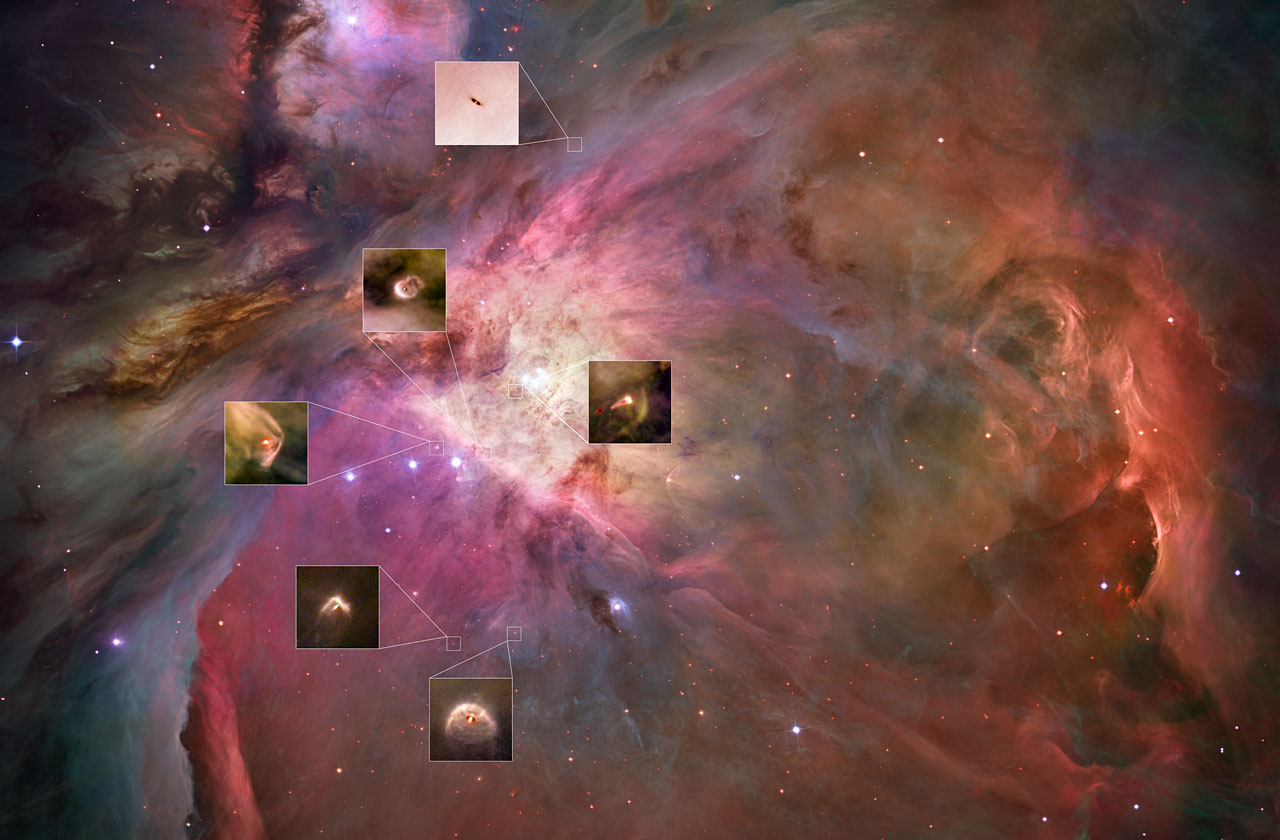
\includegraphics[width=\linewidth]{HST_Orion_proplyds.jpg}
  \captionof{figure}{Proplyds in the Orion Nebula. The closer a proplyd is to a large, bright star, the more visibly windswept it is. Image courtesy of the Hubble Space Telescope Treasury Program on the Orion Nebula (\cite{Robberto2013})}
  \label{fig:HST_ONC}
\end{figure}



The nearest high-mass SFR to us is the Orion Nebula Cluster (ONC), 389 pc away. The Hubble Space Telescope was the first to dedicate significant time to the ONC, producing an abundance of iconic and awe-inspiring images the cluster and of the disks it hosts \citep{Ricci2008}. These studies have guided many subsequent observations, including many in the radio. Many of the cluster's protoplanetary disks (or proplyds, as those in the ONC are called) are visibly teardrop-shaped, tailing away from the cluster's biggest and brightest stars, which are pushing a four parsec-diameter bubble outward at 13 \kms \citep{Pabst2019}. Images like Fig \ref{fig:HST_ONC}, showing disks being pushed away from nearby bright stars, and countless others demonstrate the harsh environment that these young disks exist in. Indeed, the influence of these large stars has already been demonstrated, both in their affect on mass-loss rate and mass distribution. Statistically-significant anti-correlations between disk mass and proximity to the ONC's central O star, $\theta^1$ Ori C, have been shown using both data from the SMA \citep{MannWilliams2009} and ALMA \citep{Mann2014,Ansdell2017,Eisner2018}.


Furthermore, both observations \citep{HenneyODell1999} and modeling \citep{Haworth2016} characterizing mass-loss rates for these proplyds in the Orion Nebula have found rates of $\dot{M} \approx 10^{-7}-10^{-5}$ M$_{\odot}$ yr$^{-1}$, implying that a typical disk (i.e. one of MMSN-scale, or $\sim0.01$ M$_{\odot}$) should be fully dispersed before giant planets could form \citep{Hubickyj2005} and before they could reach the inferred age of the disk-hosting stars in the ONC of $\approx$ 2 Myr \citep{Reggiani2011}.

% $''$There are probably more recent references for all of these.  Did you know that you can do a backwards citation search in ADS, and see which papers cited a paper of interest?  If it’s a paper with a ton of citations (as many of these are) it can be tough to sort through the results, but reading the titles can help, and then looking at the introductions of the most recent papers to see which other papers they cite. $''$ REWORK

 
Despite all this, not only do we still see disks, but we still see significant planet-forming potential in the Orion Nebula, potential that is comparable to that of other low-mass SFRs. A full 30\% of disks surveyed in the ONC have disks with masses greater than or equal to the MMSN \citep{Mann2014}, falling comfortably between $\rho$ Ophiuchus' 29\% \cite{AndrewsWilliams2005} and Taurus' 37\% \citep{AndrewsWilliams2007}.


However, since all these surveys are based exclusively on the analysis of dust continuum emission, the comparison is profoundly hamstrung by its reliance on assumptions of gas/dust ratios drawn from the ISM literature. This means that the resulting understanding of the gas masses in these regions is directly proportional to that 100:1 gas/dust ratio, a value that is almost certainly not accurate (as discussed in \S\ref{chap:continuum}). The consequences of this assumption are signficant, since a disk's gas mass directly determines its giant planet forming potential both by setting the amount of raw material available to the forming planet as well as by influencing the environment's turbulence profile and planets' migratory patterns within the disk. Furthermore, these continuum surveys cannot reveal these disks' chemistries and the environmental influences that likely affect them, instead simply assuming solar composition. Together, these assumptions regarding both the total gass mass as well as its composition result in a heavy asterisk accompanying any claims we make about the birth and evolution of protoplanetary disks in high-mass SFRs. To solve this, we must understand the chemical make up of these disks, and for that we need studies of line emission.




\citet{Mann2014} made the first line-emission survey of the Orion proplyds as part of ALMA's Cycle 0 Early Science operation. The survey studied 22 disks in four molecular lines (HCO$^+$, HCN, CO, and CS) and $856 \mu$m continuum, and calculated each disk's dust mass from the continuum emission. Since then, only one of the disks has had its line data analyzed. \cite{Factor2017} performed an analysis of the radial distribution of one of the disks' gas by modeling emission from the lines to try to understand the chemical abundance and physical structure of different molecules in the disk. This fitting process was performed on three of the four molecular lines (as CS had insufficient signal to produce meaningful constraints).

In the study, the authors found several unexpected features: their measurement of the disk's HCN abundance was higher than expected (although HCO$^+$ and CO abundances were consistent with literature values from low-mass SFRs), their mass measurement for the central star was inconsistent with the previously-determinded spectral type, and they found a spatially unresolved high-velocity excess emission feature in the HCO$^+$(4-3) and CO(3-2) lines, with a positional offset from the central star. For this emission feature, they found that the source was blue shifted by $-6.2$ km s$^{-1}$ relative to the systemic velocity, had a position consistent with a $60\pm20$ AU Keplerian orbit, and had an inferred H$_2$ mass of 1.8-8 M$_\text{Jup}$. They determined that the excess of emission was caused by a local density and/or temperature fluctuation in the inner disk, indicating that it was not a jet or cloud contamination. The authors propose that this could be the result of young Mars-sized bodies, collisions between particles trapped in mean motion resonance by a giant planet, magnetic-field-induced zonal flows, or planet formation.


These unexpected results demonstrate the need for further analysis of disks in this survey. The binary system that is the subject of this thesis is drawn from the same survey, representing the second and third ONC proplyds to have their temperature and density profiles characterized.





\section{d253-1536: A Misalgined Binary System}

The subject of this thesis is the system d253-1536, a binary of pre-main sequence stars in the M43 region of the Orion Nebula Cluster. Each star has its own proplyd. The stars' projected separation is somewhat atypically wide (approximately 428 au), and their rotational axes are misaligned. Each star in the system has its own disk, henceforth called disk A and disk B (east and west, respectively, in all images of the system\footnote{The reader will recall that this corresponds to disk A being on the left and disk B on the right of all images, since east and west are inverted in celestial coordinates relative to our familiar geographic ones.}).

\subsection{Local Environment \& Features}
Many previous surveys have studied disks in the famous M42, or Orion Nebula, which lies adjacent to M43, and particularly the Trapezium cluster, a region near M42's brightest star O-star $\theta^1$ Ori C. \citet{Mann2014} found a statistically significant correlation between disk mass and distance from $\theta^1$ Ori C in a study of 70 proplyds (Fig. \ref{fig:onc_disk_relations}), particularly within 0.03 pc of the star, where there is a lack of disks more massive than $3 M_\text{jup}$. These disks are also truncated in radial extent, with no disks extending out past 60 AU in this region \citep{Eisner2018}.


\begin{figure}[htp]
  \hspace*{\fill}%
  \subcaptionbox{\label{fig:onc_disk_masses}}{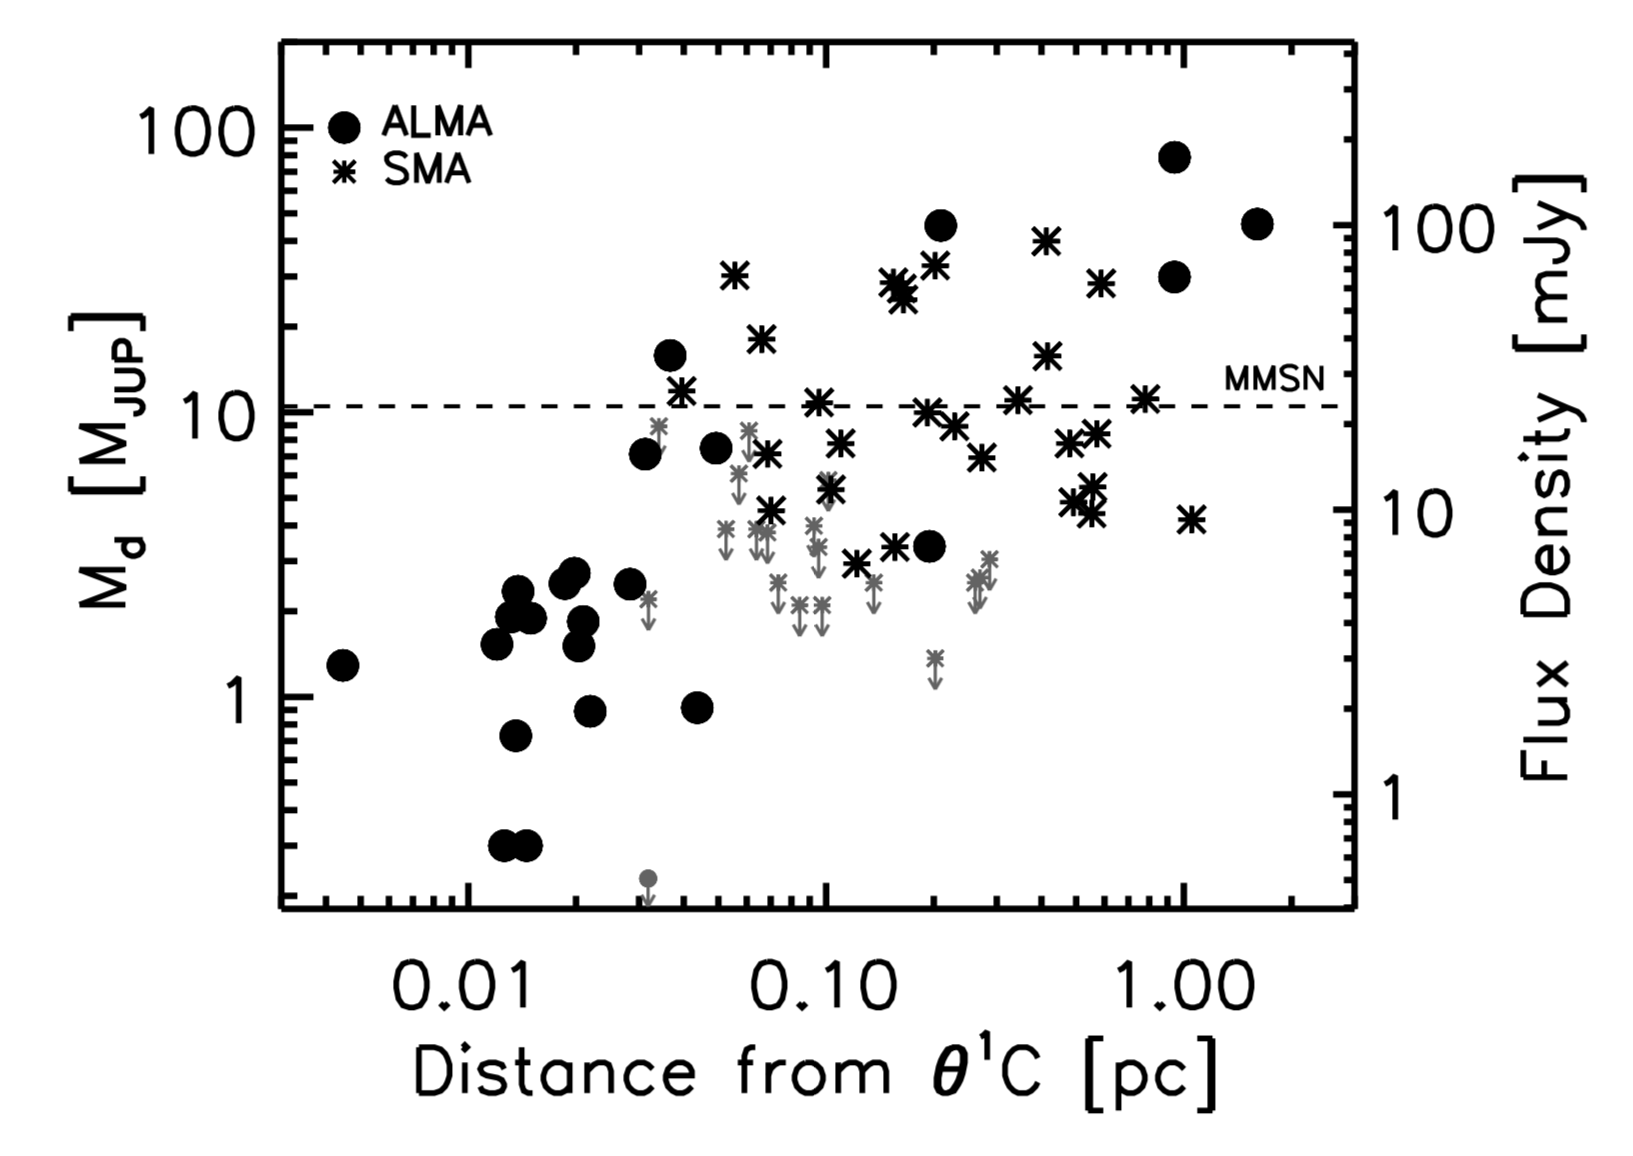
\includegraphics[width=0.52\linewidth]{onc_disk_masses.png}}\hfill%
  \subcaptionbox{\label{fig:onc_disk_radii}}{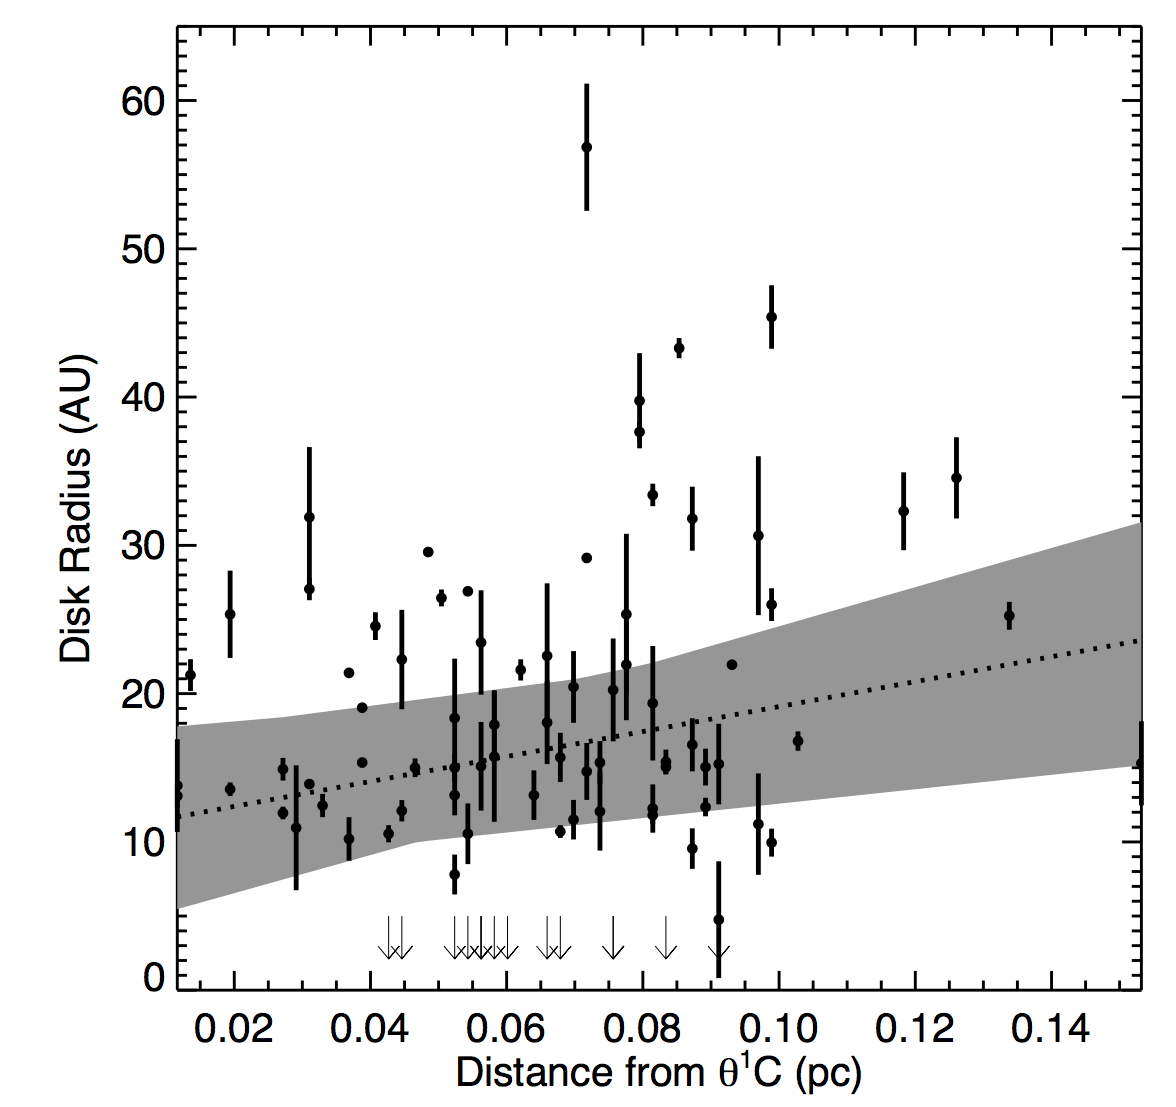
\includegraphics[width=0.38\linewidth]{onc_disk_radii.png}}%
  \hspace*{\fill}%
  \captionof{figure}{\textit{Left}: The masses of 70 ONC proplyds are plotted against their projected distance from the Orion Nebula's central O-star, $\theta^1$ Ori C, drawn from surveys from ALMA and the SMA \citep{Mann2014}. Grey markers indicate $3 \sigma$ upper limits for non-detections. The dashed line at 10 M$_\text{Jup}$ indicates the minimum-mass solar nebula. As is clear from this plot, a statistically-significant correlation was found between disk mass and distance from $\theta^1$ Ori C. \textit{Right}: Radius is also affected by proximity to $\theta^1$ Ori C \citep{Eisner2018}}
  \label{fig:onc_disk_relations}
\end{figure}


However, because of M43's separation from the Trapezium cluster (it lies $\geq$ 1 pc to the cluster's north; see Fig.\ref{onc_map}), disks in this region do not experience the same levels of photoevaporation. M43 has only one large emitter, NU Ori, which is a triple-star system whose main component is a B-stype star. d253-1536 is wrapped in an ionization bow shock, HH 668 A (Fig.\ref{fig:v2434ori_smith05}), about 1" to the system's west and facing towards NU Ori, but otherwise the system shows no signs of influence from giant stars, whether in photoevaporation or in morphological influences \citep{MannWilliams2009}.

The misalignment of the disks' rotational axes is fairly typical of wide binaries like this one \citep{Williams2014}. The frequency with which these wide binaries present such misalignment indicates that wide binaries likely do not form in large, co-rotating structures, and emphasizes the importance of gas turbulence and inter-stellar interactions for young stars.


The system's larger disk, disk A, has a large jet emanating from it in observations in the optical made with HST \citep{Smith2005}. However, since the jet is not visibile in the radio, we make no attempt to discuess, model or explain it.


\begin{figure}[t]
\centering
  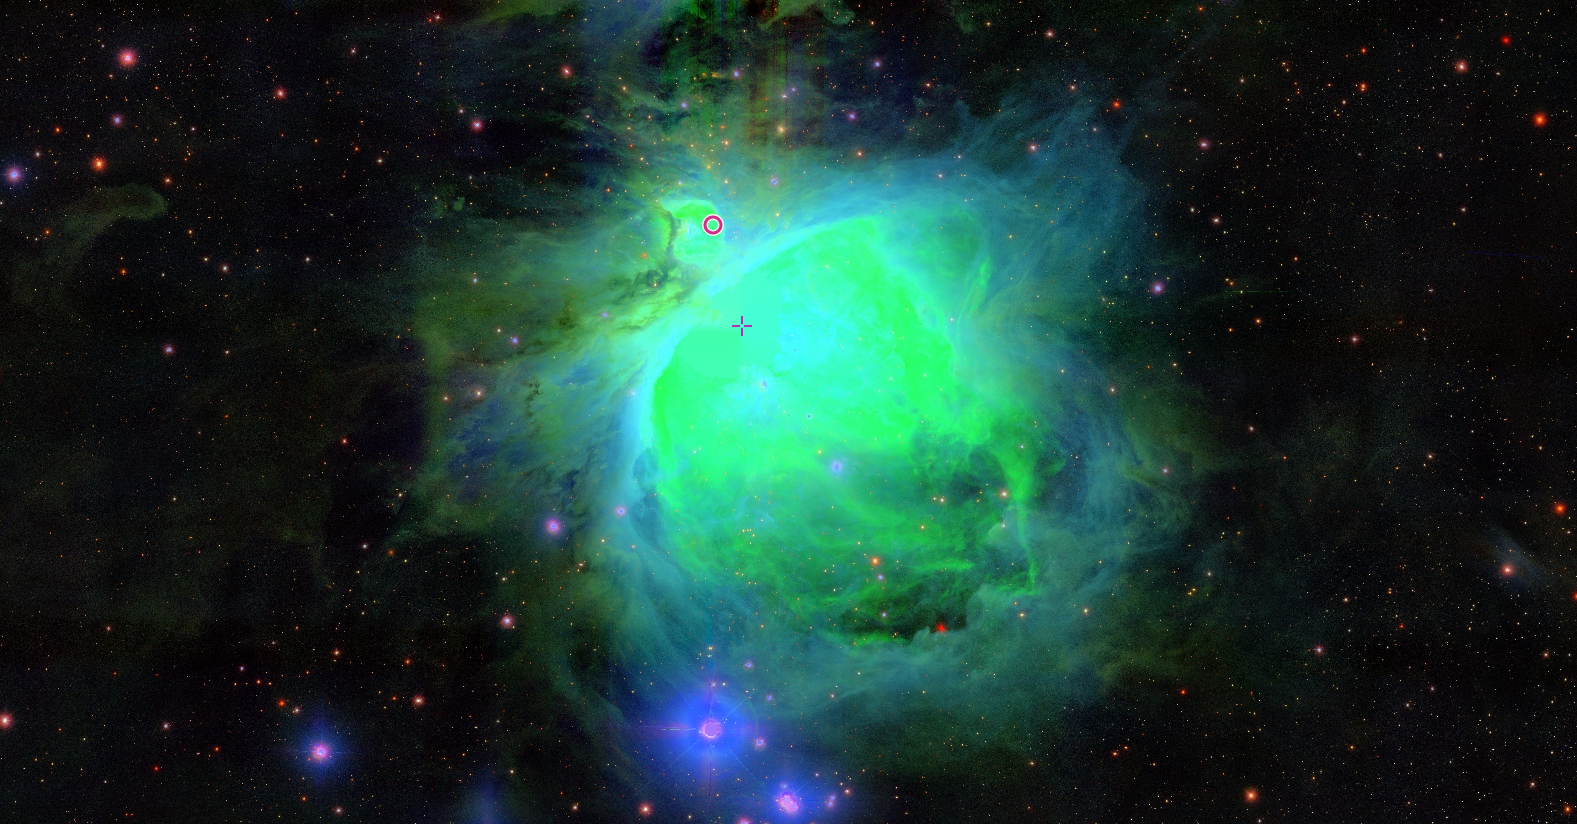
\includegraphics[width=\linewidth]{ONC_Map.png}
  \caption{M42 and M43, shown in SDSS coloring, with the locations of d253-1536 (marked with a red circle) and $\theta^1$ Ori C (marked with crosshairs), the heart of the Trapezium cluster. Map created in AladinLite viewer. Because of the large separation between d253-1536 and Trapezium, the disks don't show the same obvious marks of influence from OB stars seen in other disks closer to the heart of M42.}
  \label{fig:onc_map}
\end{figure}
%
% \begin{figure}[t!]
% \centering
%   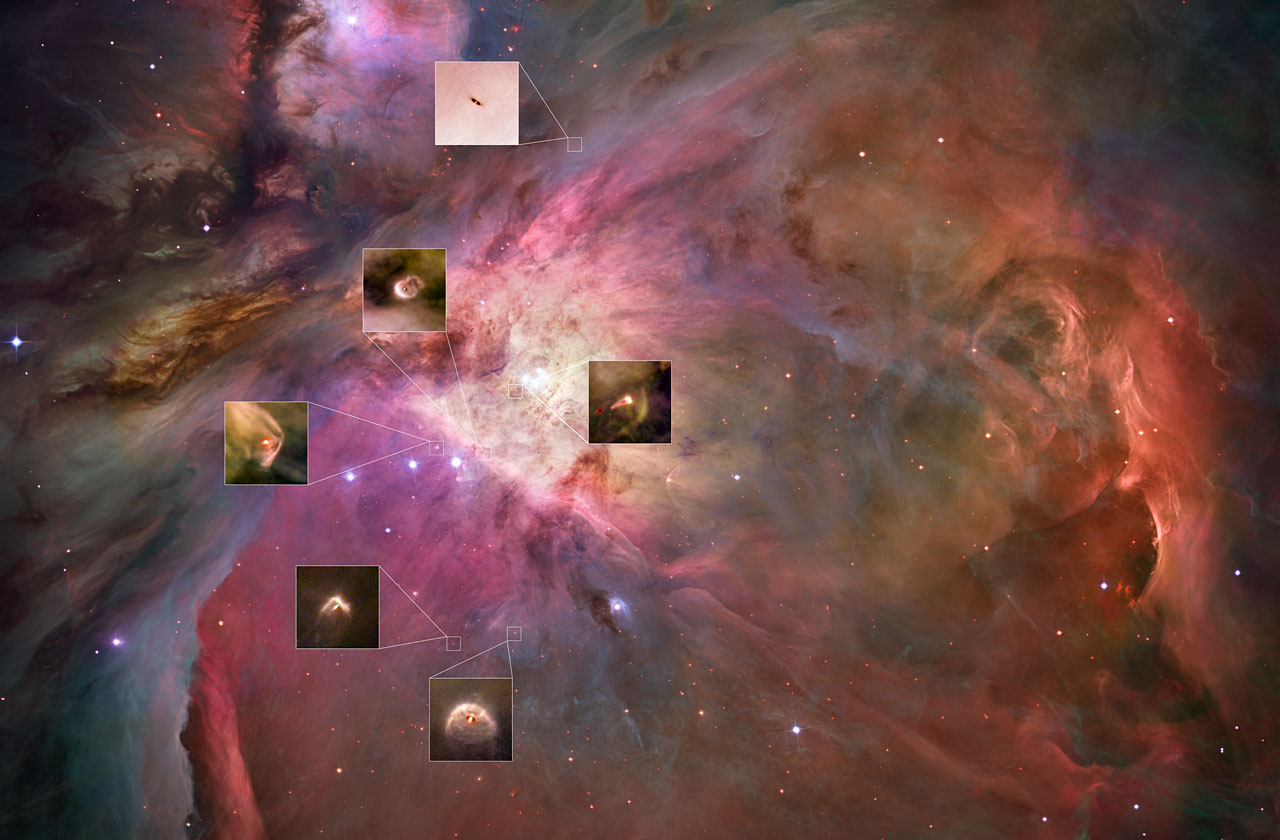
\includegraphics[width=\linewidth]{HST_Orion_proplyds.jpg}
%   \captionof{figure}{Proplyds in the Orion Nebula. The closer a proplyd is to a large, bright star, the more visibly windswept it is. Image courtesy of the Hubble Space Telescope Treasury Program on the Orion Nebula (\cite{Robberto2013})}
%   \label{fig:HST_ONC}
% \end{figure}




\subsection{Previous Observations}

\begin{figure}[htp]
  \hspace*{\fill}%
  \subcaptionbox{\label{fig:v2434ori_smith05}}{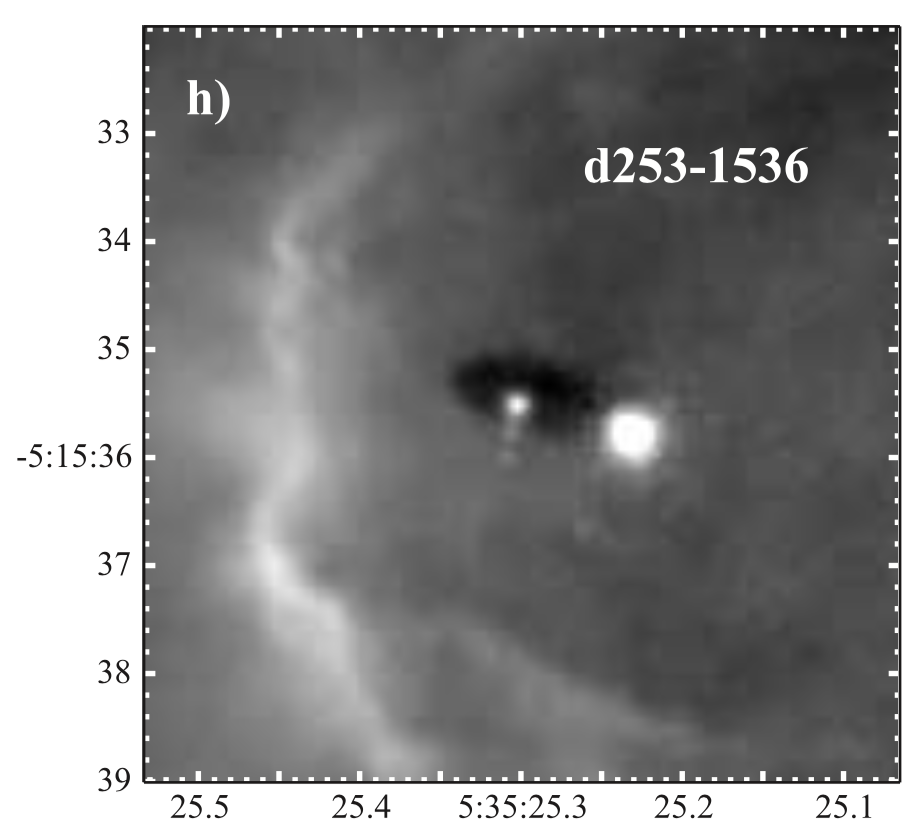
\includegraphics[width=0.33\linewidth]{V2434Ori_Smith05-2.png}}\hfill%
  \subcaptionbox{\label{fig:v2434ori_mann09}}{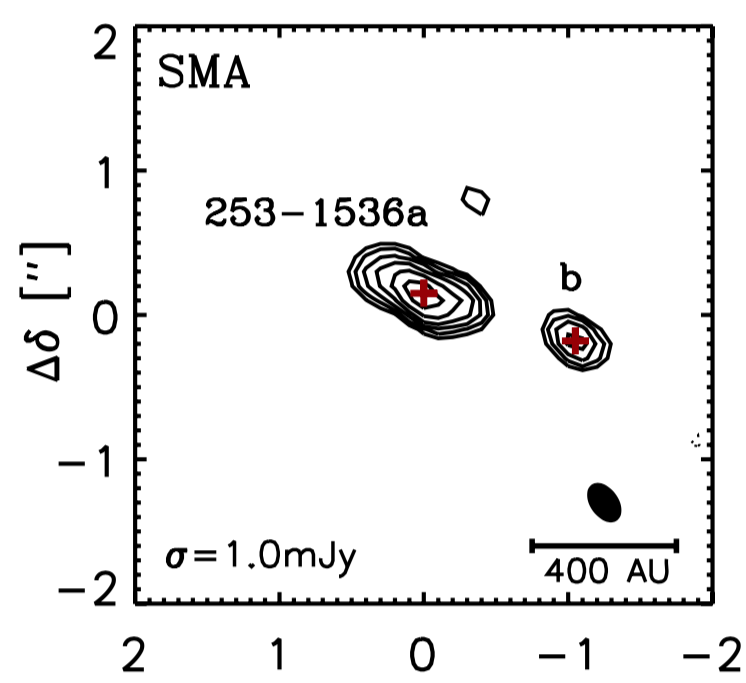
\includegraphics[width=0.33\linewidth]{V2434Ori_Mann09.png}}\hfill%
  \subcaptionbox{\label{fig:v2434ori_ricci11}}{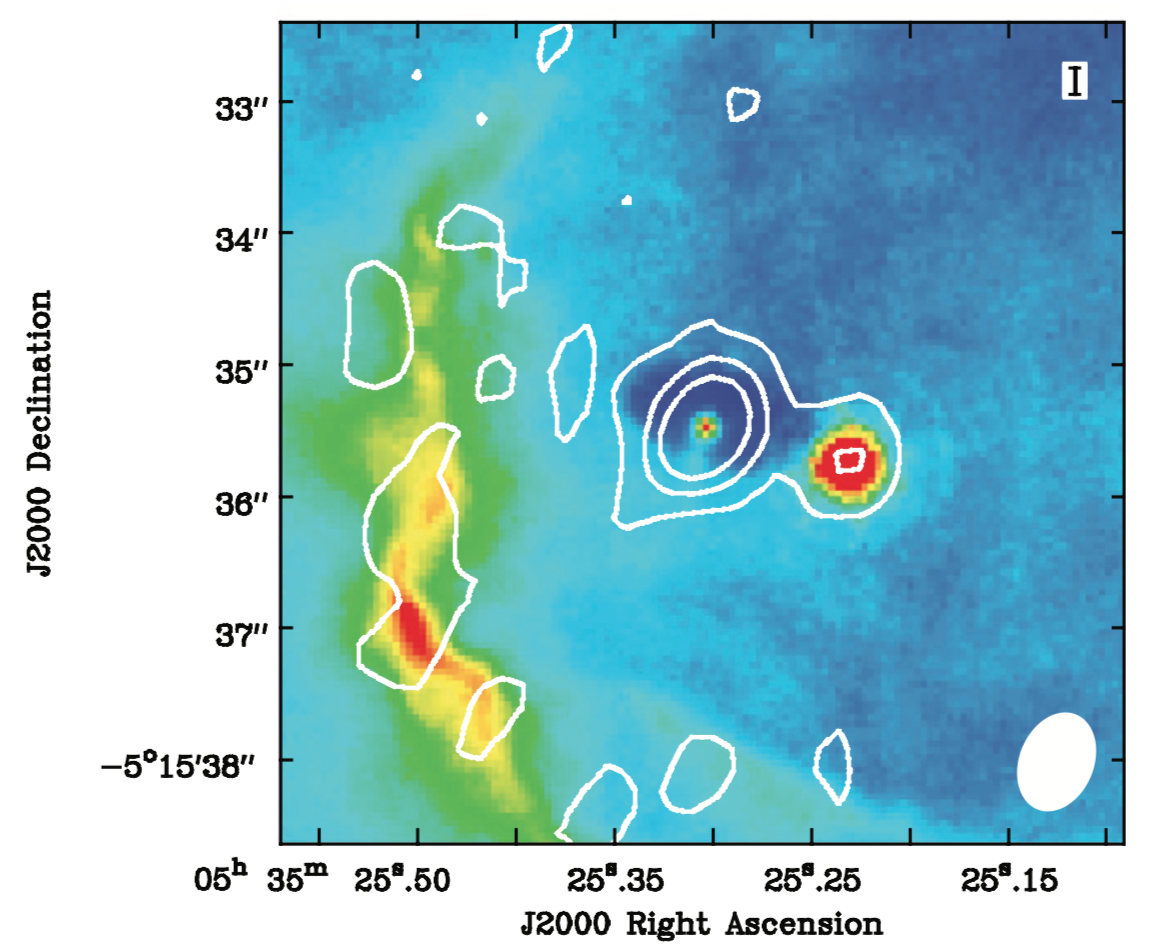
\includegraphics[width=0.33\linewidth]{V2434Ori_Ricci11.png}}\hfill%
  \hspace*{\fill}%
  \captionof{figure}{Images of V2434 Ori taken from \citet{Smith2005} on HST (Fig. \ref{fig:v2434ori_smith05}), \citet{MannWilliams2009} with the SMA at 880 $\mu$m (Fig. \ref{fig:v2434ori_mann09}), and \citet{Ricci2011} with the EVLA at 7mm (Fig. \ref{fig:v2434ori_ricci11}). The ionization front is clearly visible in both the HST and EVLA observations, and the jet from disk A is visible in the HST image.}
\end{figure}

First observed by \citet{Smith2005} using the Hubble Space Telescope, the authors took interest in what they saw as a binary system containing one star without a disk and one star embedded in a proplyd with a large jet and exhibiting tidal interactions with its companion (Fig \ref{fig:v2434ori_smith05}). \citet{MannWilliams2009} used 880 $\mu$m continuum measurements to estimate dust masses of the disks to be 0.066 M$_{\odot}$ and 0.018 M$_{\odot}$, for disks A and B respectively, making d253-1536a the most massive disk measured in the ONC, significantly larger than the Cluster's second largest disk at 0.034 M$_\odot$ and adding credence to the theory that $\theta^1$ Ori C is likely responsible for the truncation of disk masses in the Trapezium cluster. Subsequent detections at 7mm by \cite{Ricci2011} indicated that both disks are hosts to substantial populations of large dust grains (\ref{fig:v2434ori_ricci11}), although the distributions of grain sizes are different in the two disks. The same study also spectral typed the host of d253-1536b to be an 0.4 M$_\odot$ M2 star and a 3.5 M$_\odot$ G2 for d253-1536a's host star. This mass ratio of around 9:1 is somewhat atypically high for pre-main sequence binaries \citep{Duchene2013}.


\begin{figure}[htp]
  \hspace*{\fill}%
  \subcaptionbox{\label{fig:m1map_hco}}{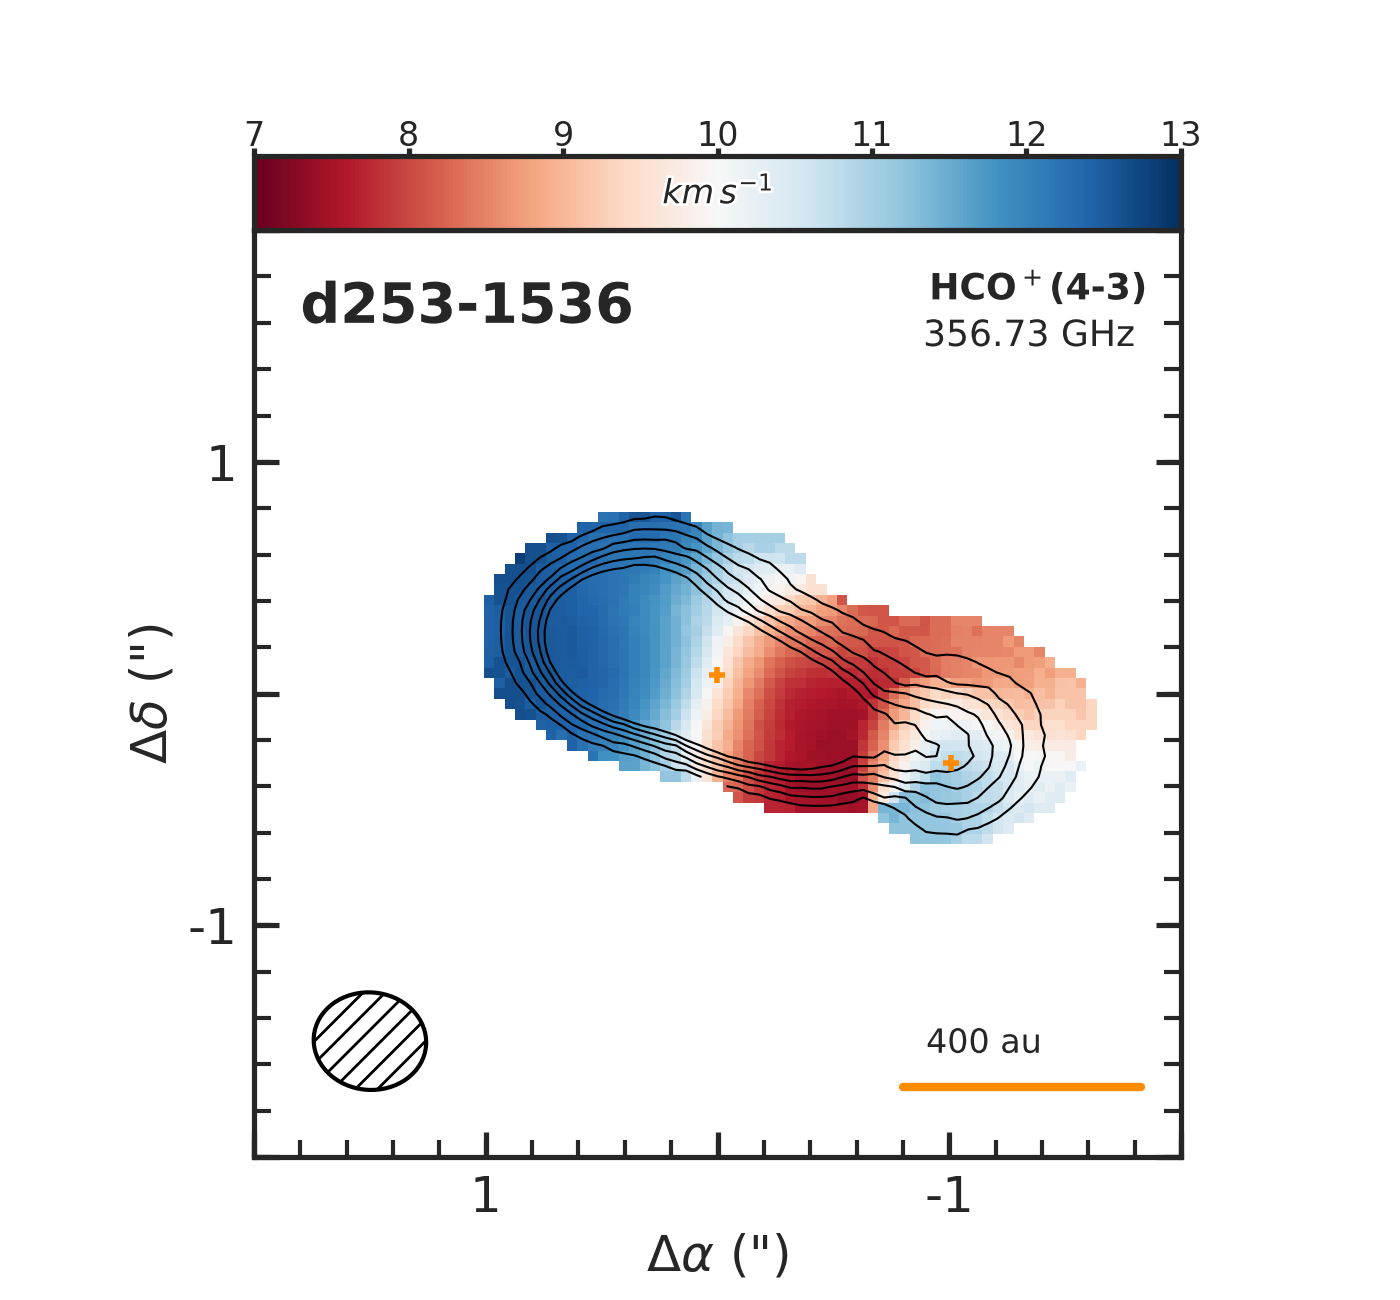
\includegraphics[width=0.25\linewidth]{moment1_hco-data.pdf}}\hfill%
  \subcaptionbox{\label{fig:m1map_hcn}}{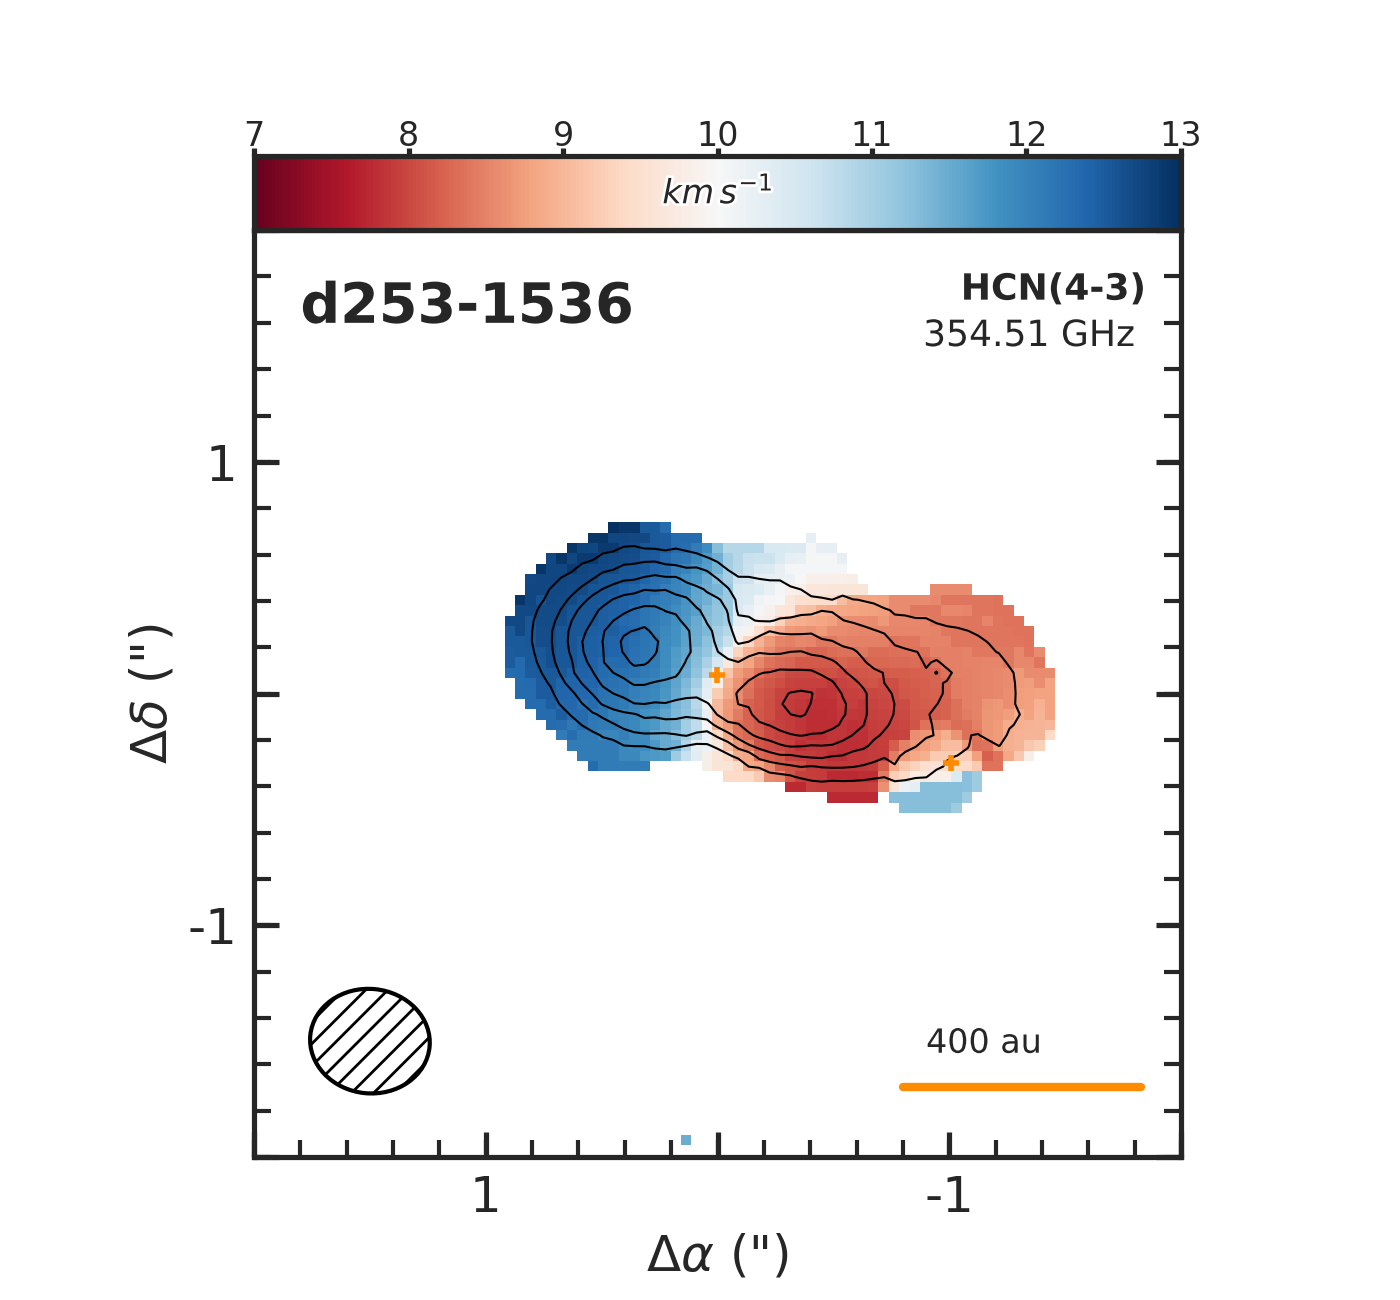
\includegraphics[width=0.25\linewidth]{moment1_hcn-data.pdf}}\hfill%
  \subcaptionbox{\label{fig:m1map_co}}{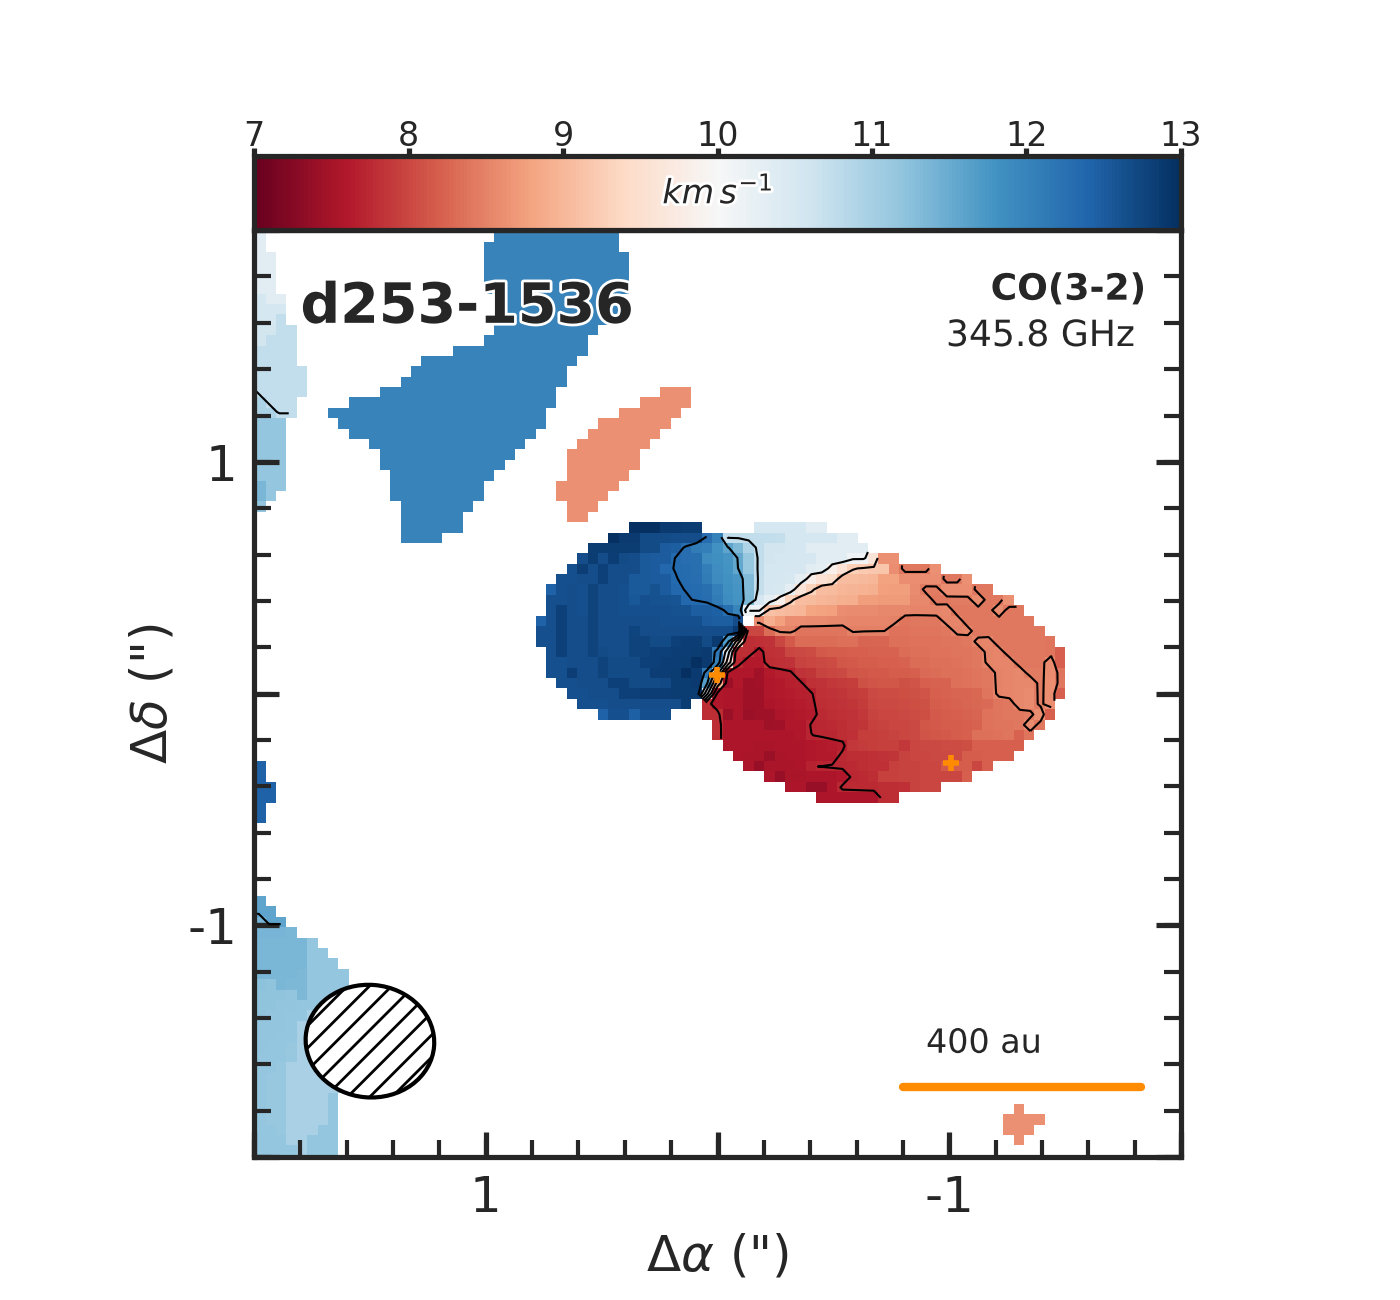
\includegraphics[width=0.25\linewidth]{moment1_co-data.pdf}}\hfill%
  \subcaptionbox{\label{fig:m1map_cs}}{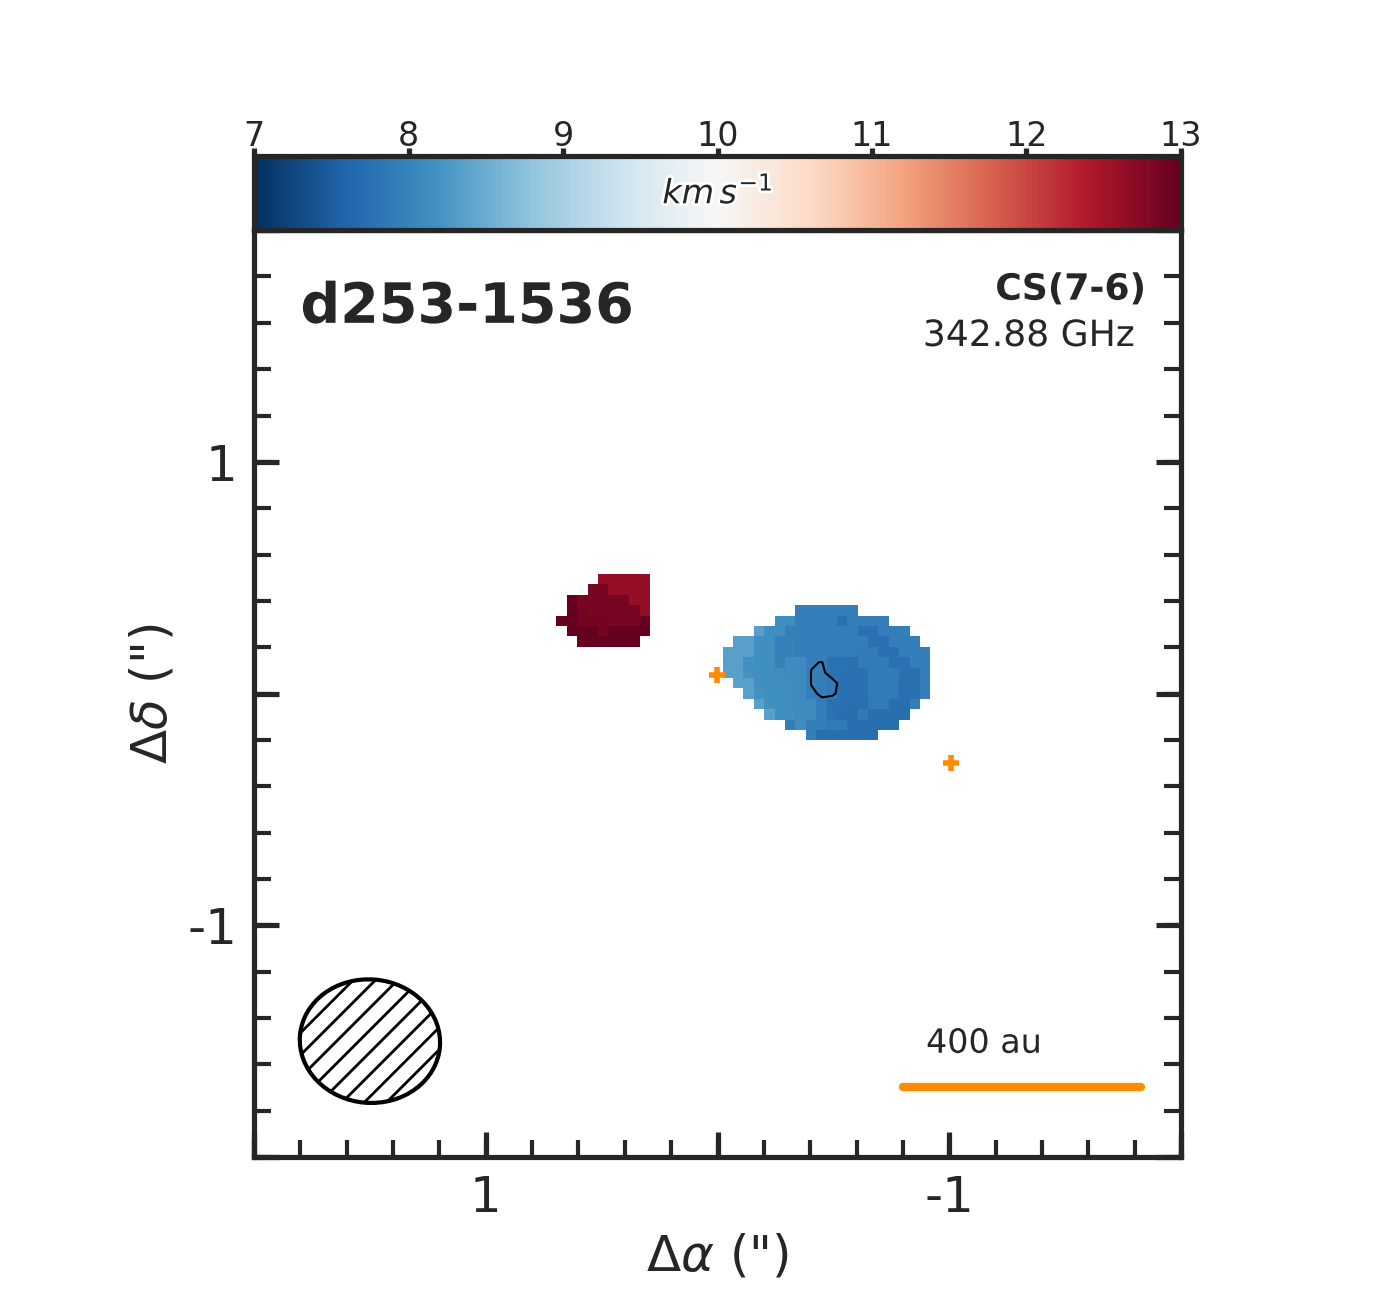
\includegraphics[width=0.25\linewidth]{moment1_cs-data.pdf}}\hfill%
  \hspace*{\fill}%
  \label{fig:m1map}
  \captionof{figure}{Moment-1 maps of HCO$^+$(4-3), HCN(4-3), CO(3-2), and CS(7-6) emission (left to right) in the present study's proplyds, observed with ALMA's Band 7. Each map shows intensity-weighted velocity, which allows us to trace the disks' kinematics. REWORK: considering making this a 2x2 grid, instead of 4 across.}
\end{figure}
% Need a more detailed figure caption.  What do all of the symbols on the map mean?  What object are we looking at?  With which telescope?  AT which frequency?  (Which transitions are these, specificaly?)  What do the contours mean?  What are the colors?  Take a look at some papers for examples of what information should go into a figure caption.


The system was observed in an ALMA survey of 22 proplyds in M43 by \citet{Mann2014} in four molecular lines (HCO$^+$(4-3), HCN(4-3), CO(3-2), and CS(7-6); Fig \ref{fig:m1map}), and preliminary fits of the system's kinematics in the HCO$^+$(4-3) line were made by \citet{Williams2014}. Using continuum observations alone and assuming canonical values for temperature, dust opacity, and gas-to-dust ratio, they found disk masses of 0.074 M$_{\odot}$ and 0.028 M$_{\odot}$ for disks A and B, respectively, larger than the previous values. They found an inclination for disk A of $i_A \sim 65^\circ$, but did not resolve disk B and thus were unable to determine its inclination. They found systemic LSRK velocities of 10.55 and 10.85 km/s for the two disks, which are close enough to be well within the escape velocity that the authors calculated for a disks at their projected separation of 440 AU of 2.5 km/s, indicating that the binary is bound. This similarity in systemic velocity also indicates that the binary's orbital plane is likely close to face-on.



With our high resolution observations of gas line emission, we aim to determine the temperature, density, and chemical profiles of the system, as well as refining the mass estimates for both disks and host stars. With this information in hand, we will examine this disk's characteristics in the context of previously studied disks in the Taurus and $\rho$ Ophiuchus star forming regions, as well as comparing it to the disk studied by \citet{Factor2017}, and evaluate the disks' planet forming potentials.






\section{Summary of Contents}

In this work we characterize ALMA observations of two young protoplanetary disks in the d256-1536 system. Observations and data reduction are described in \S2. In \S3, data and basic analysis are presented. Descriptions of modeling and fitting techniques are discussed in \S4, and in \S5, best-fit parameters are discussed and contextualized, as well as unexpected features maybe.
% Tossing a REWORK tag here so that I remember to get rid of that maybe.
% Also maybe combine the last paragraph of the previous section and Summary of Contents? They seem redundant.





















% The End
